\documentclass{sig-alternate}
\setlength{\pdfpagewidth}{8.5in}
\setlength{\pdfpageheight}{11in}

\usepackage{graphicx}
\usepackage{subfigure}

\newcommand{\fref}[1]{Figure \ref{#1}}

\newcommand{\SJ}{TOUCH}
\newcommand{\newSJ}{EVERGREEN}
\newcommand{\dSJ}{dTOUCH}
\newcommand{\cSJ}{cTOUCH}
\newcommand{\reSJ}{reTOUCH}
\newcommand{\rereSJ}{re*TOUCH}

\begin{document}

\section{Experimental Evaluation}
\label{s_experimental_evaluation}

This set of experiments comprises of comparing leafsize and fanout effect on {\newSJ} variations and traversal type.

\subsection{General Setup}
\subsubsection{Hardware setup}
Laptop, Intel CORE i7, NVIDIA CUDA 5.5. Thrust library (for parallel sorting during building phase), 8 GB RAM 
\subsubsection{Algorithm parameters}
Unless specified for concrete experiment, parameters are the following:
\begin{itemize}
\item Fanout: 3
\item Leaf size: 100
\item Epsilon: 5
\item Datasets: Random Samples generated from data about Axons and Dendrites. Every experimental value is a mean of 5x5 random samples. For example, for calculating total time of joining 1000 axons with 1000 dendrites, firstly 5 random samples of axons and 5 random samples of dendrites are generated, then they are joined (25 results) and a mean result is reported.
\item Local join algorithm: SGH with dynamic grid \\
($(\frac{Node\, MBR\,  volume}{Average\,  Assigned\, Object\,  volume})^{1/3}$)
\item First tree assignment probability (For dTOUCH):\\ ${P^{B}_{T_A}}=e^{-\alpha\times\frac{l}{L_{T_A}}}\times(1-\frac{l}{L_{T_A}})$
\end{itemize}

\subsection{Leaf size}
\subsubsection{Methodology}
Leaf size is a parameter of the experiment. The default value used in other experiments is 100. In this experiment we variate leaf size from 50 to 300. Number of objects in each dataset is 2000.

\subsubsection{Observation}

\begin{figure}[htb]
    \begin{center}
        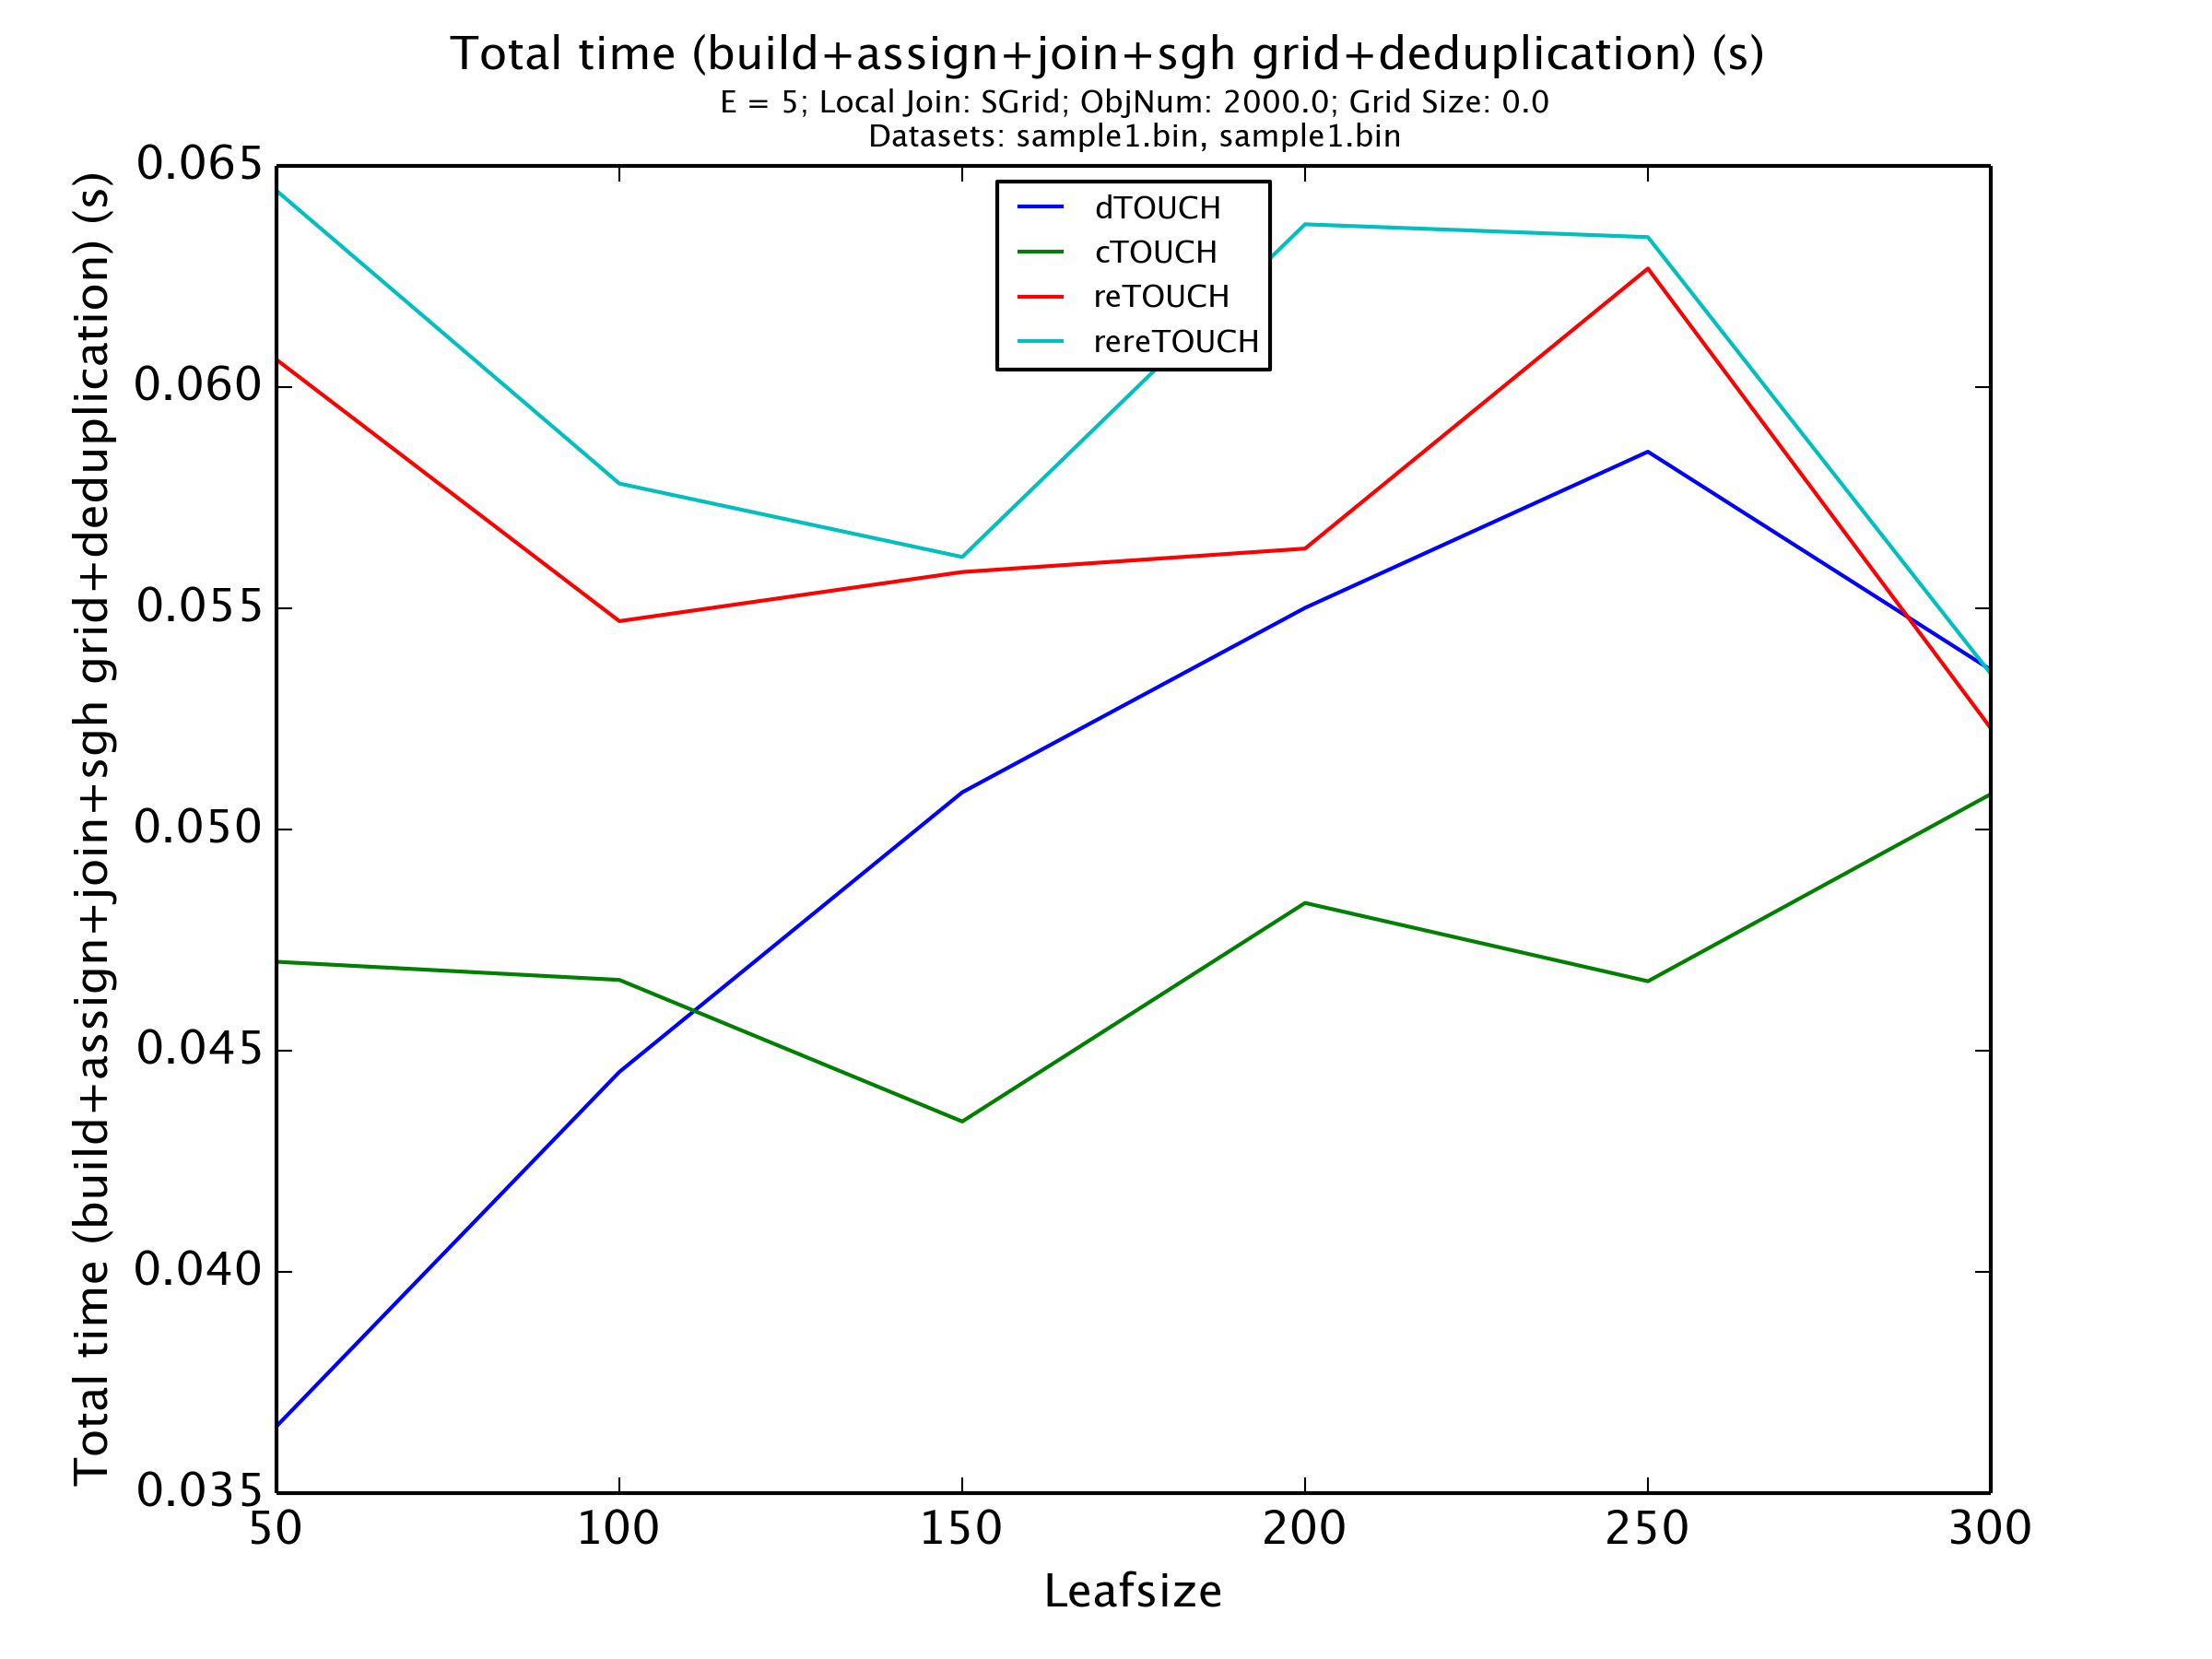
\includegraphics[width=\columnwidth]{leafsize/total}
        \caption{leafsize comparison}
        \label{fig:leafsize:time}
      \end{center}
\end{figure}

\fref{fig:leafsize:time} shows the total runtime of all the four {\newSJ} variations. We exclude {\SJ} because of distracting (worse) performance. This plot suggests:
\begin{itemize}
\item {\reSJ} and {\rereSJ}: we should run for leafsize larger than 300 to have more clue.
\item {\dSJ}: for smaller leafsize, i.e. taller tree, performs faster.
\item {\cSJ}: almost independent or a leafsize between 100 and 200 is already good enough when fanout is 3.
\end{itemize}

\begin{figure}[htb]
    \begin{center}
        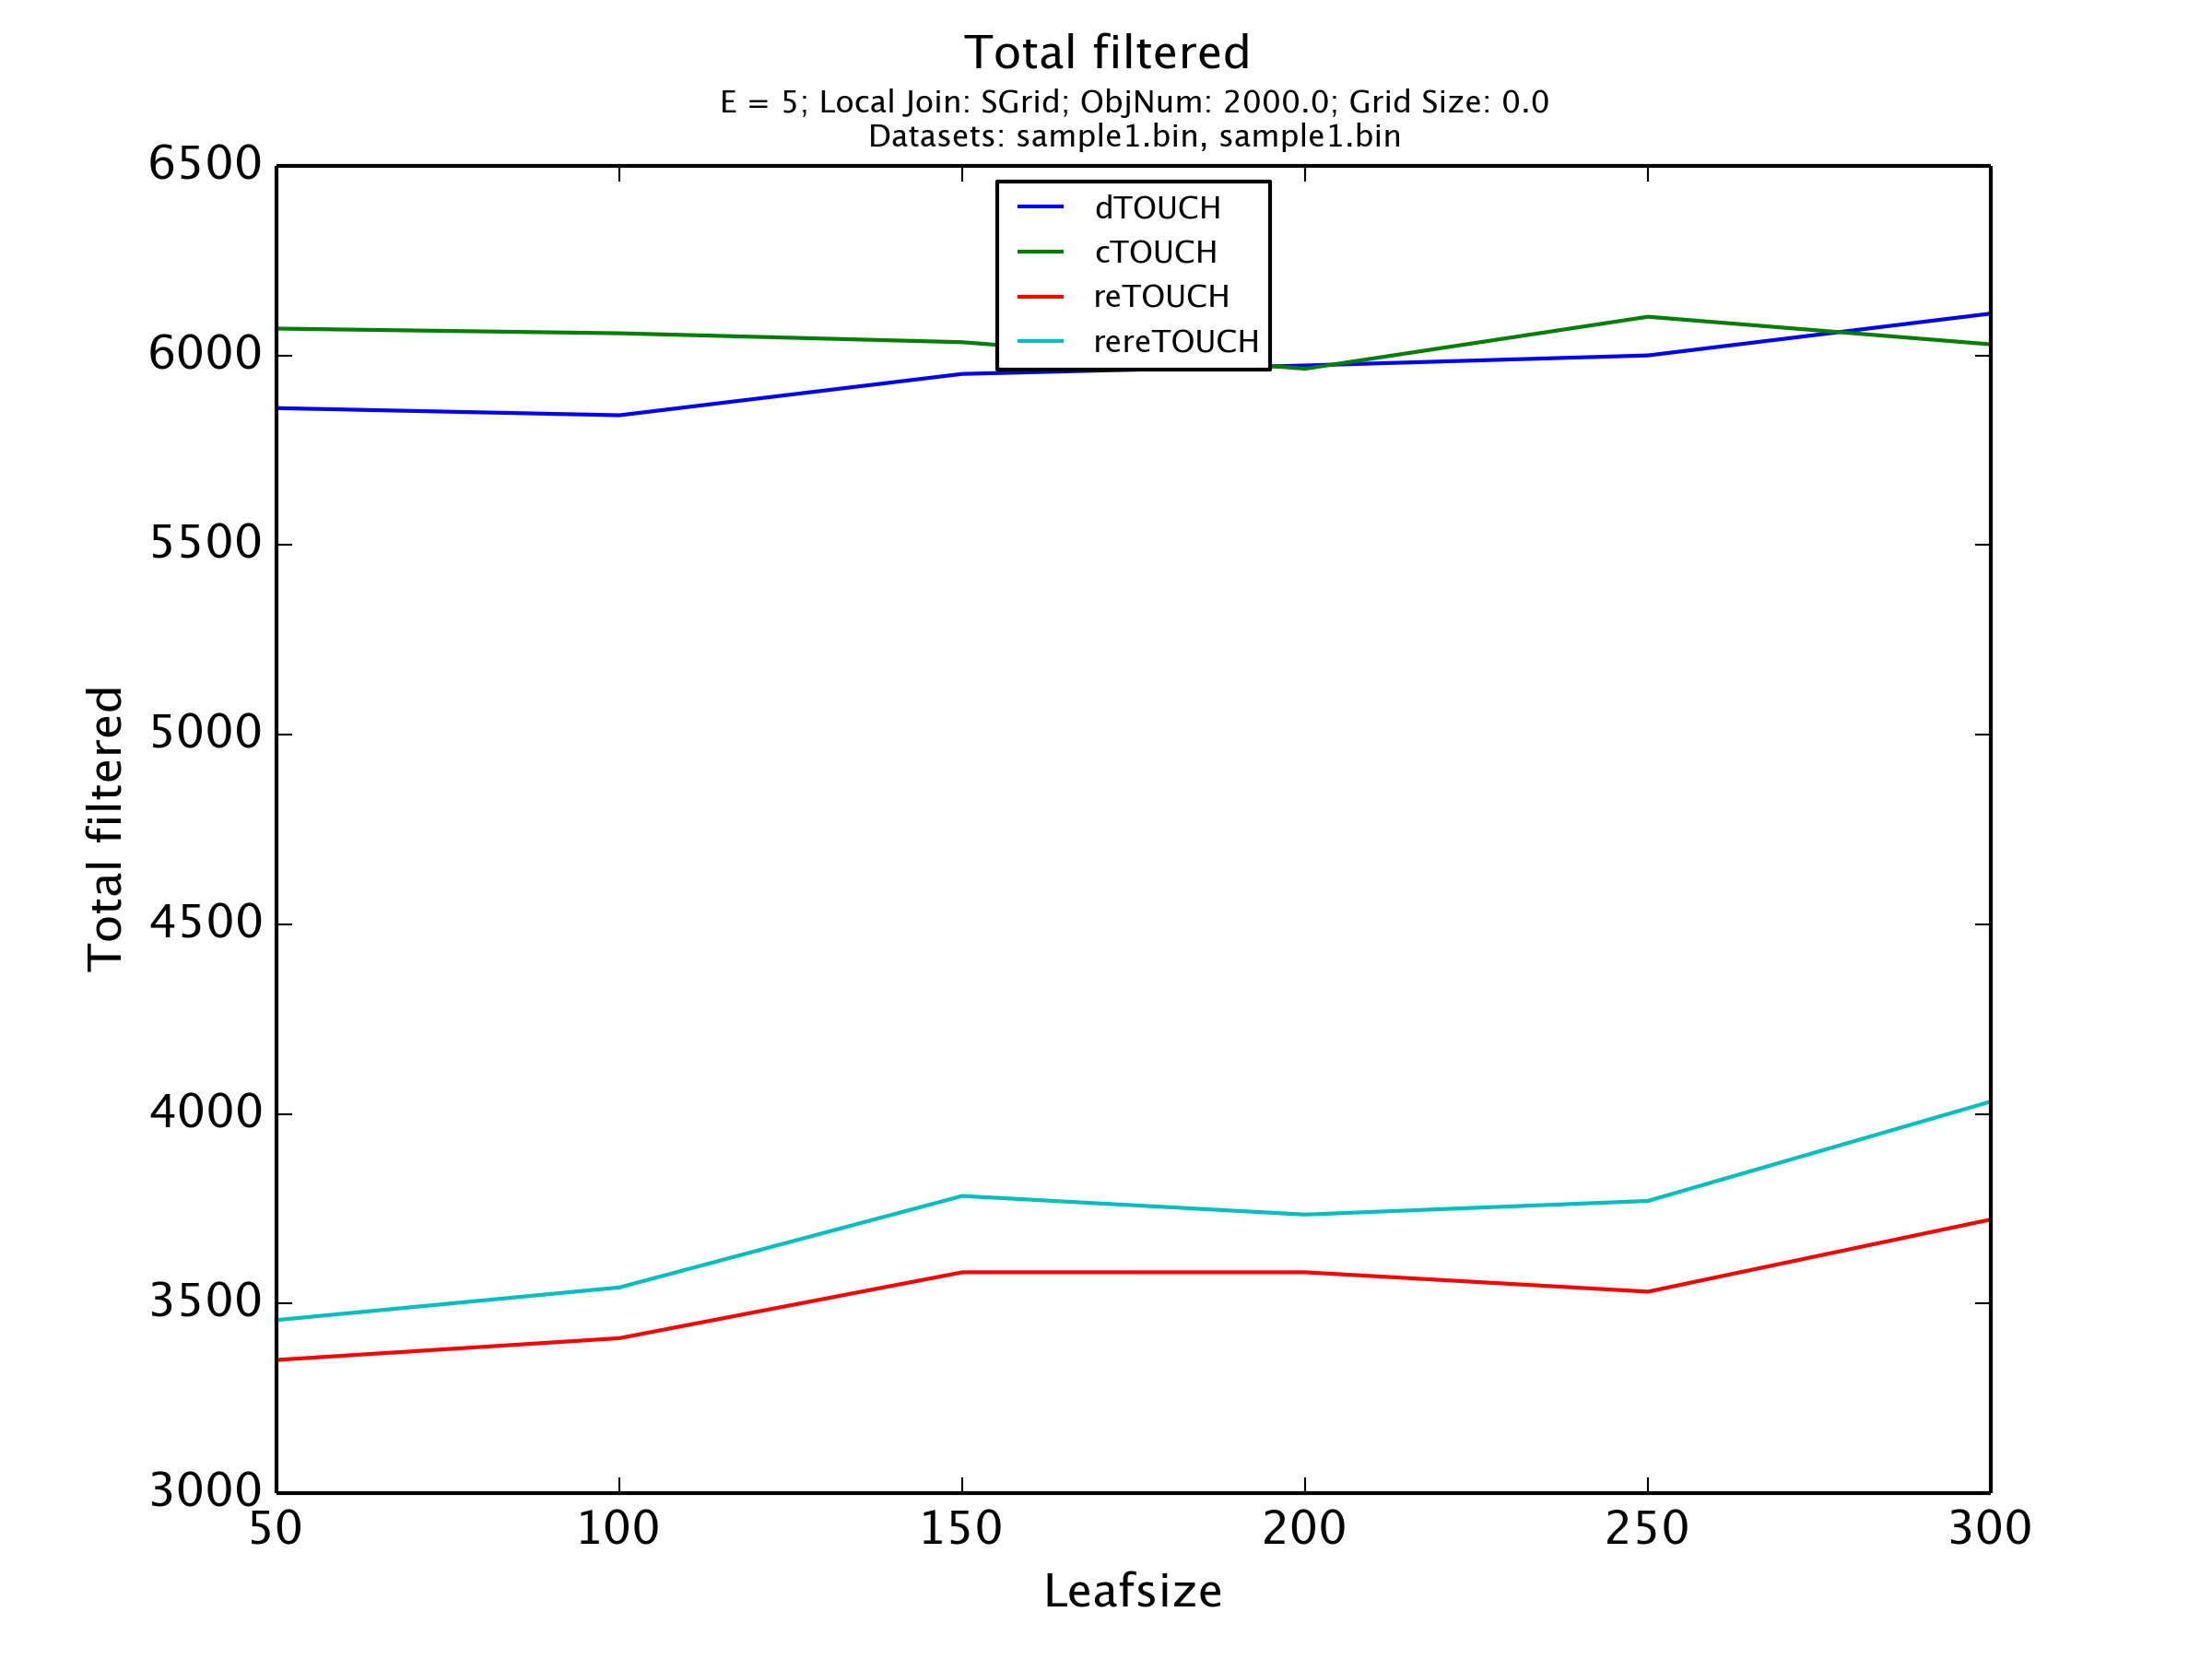
\includegraphics[width=\columnwidth]{leafsize/totalfiltered}
        \caption{leafsize comparison}
        \label{fig:leafsize:filter}
      \end{center}
\end{figure}

\fref{fig:leafsize:filter} shows the total filtering, i.e. $F_{total}$\footnote{explained in table \ref{table:terms}}. This plot suggests:
\begin{itemize}
\item {\dSJ}, {\reSJ} and {\rereSJ}: shorter tree has more filtering ability. However, we should run for leafsize larger than 300 to have more clue.
\item {\cSJ}: almost independent when fanout is 3.
\end{itemize}

\subsubsection{Conclusion}

The leafsize has very small effect on the runtime of all the variations except {\dSJ}.

\subsection{Fanout}
\subsubsection{Methodology}
Fanout is a parameter of the experiment. The default value used in other experiments is 3. In this experiment we variate leaf size from 2 to 10. Number of objects in each dataset is 2000.
\subsubsection{Observation}
\fref{fig:fanout:time} shows the total runtime of all the four {\newSJ} variations. We again exclude {\SJ} because of distracting performance. We can make following observations: 

\begin{itemize}
\item {\reSJ} and {\rereSJ}: we should run for fanout smaller 4 to have more clue.
\item {\dSJ} and {\cSJ}: the performance does not depend from fanout significantly in the observed range.
\end{itemize}

\begin{figure}[htb]
    \begin{center}
        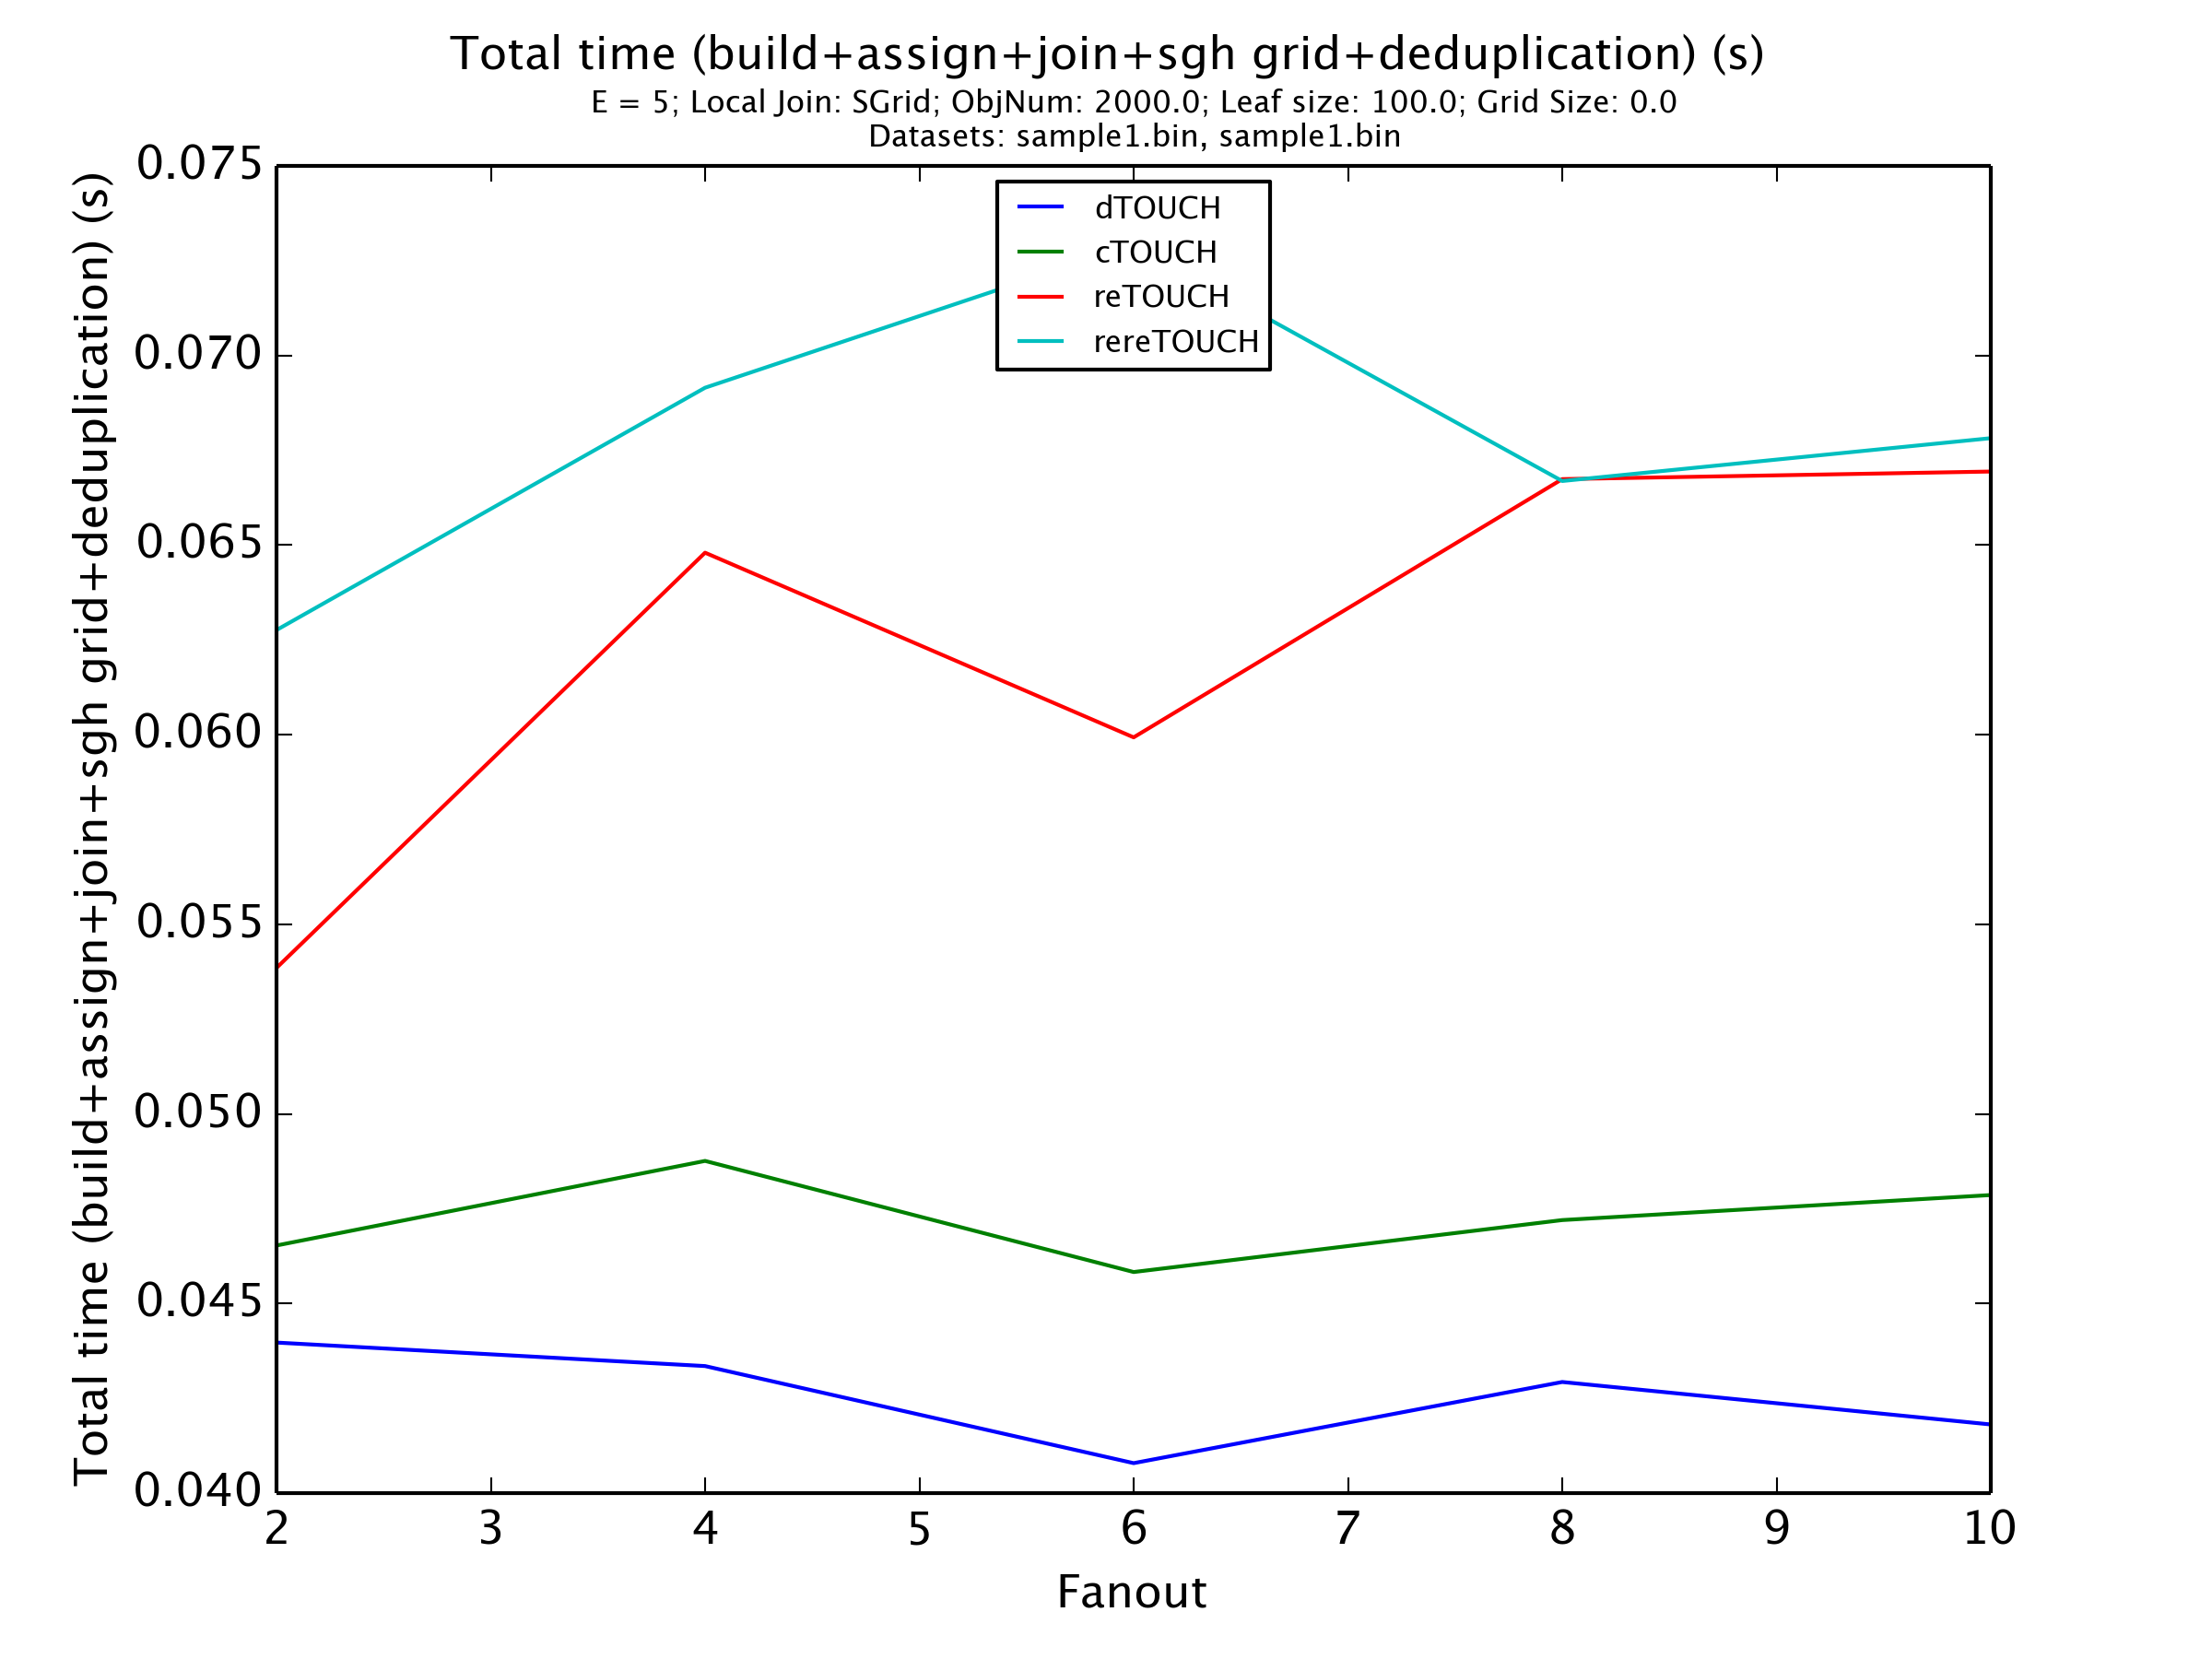
\includegraphics[width=\columnwidth]{fanout/total}
        \caption{fanout comparison}
        \label{fig:fanout:time}
      \end{center}
\end{figure}

\begin{figure}[htb]
    \begin{center}
        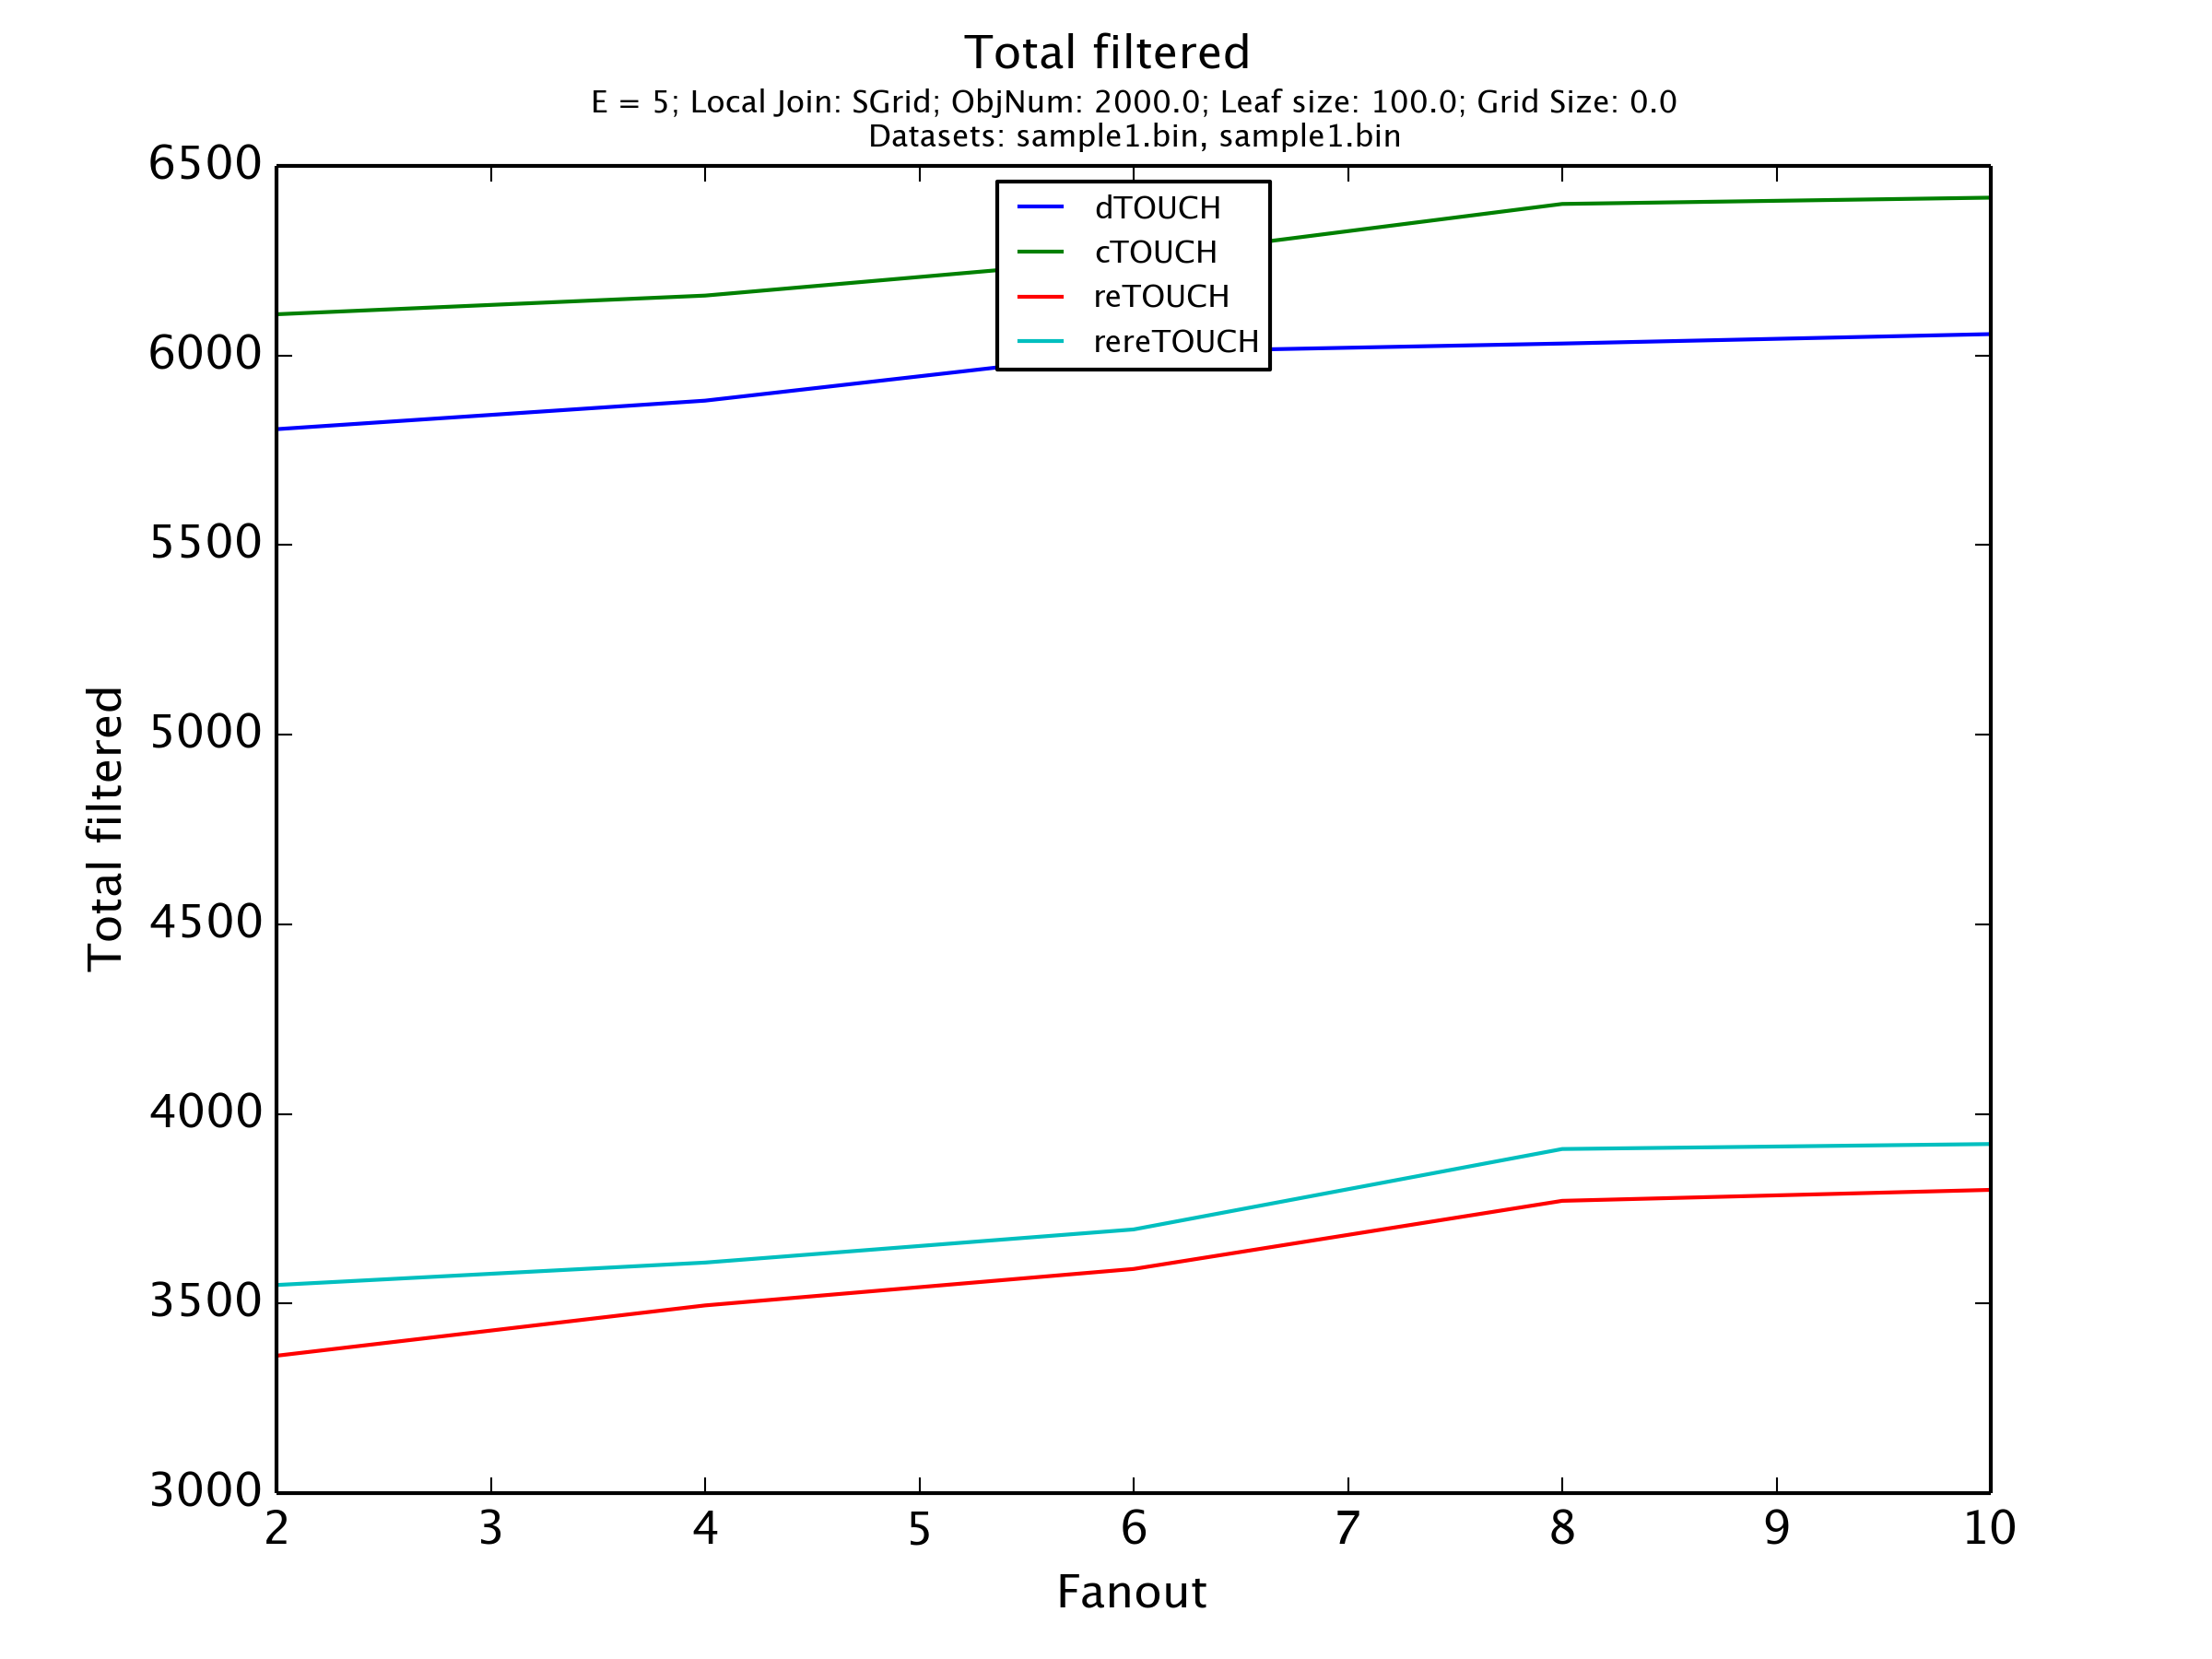
\includegraphics[width=\columnwidth]{fanout/totalfiltered}
        \caption{fanout comparison}
        \label{fig:fanout:filter}
      \end{center}
\end{figure}

For all algorithms fanout increases slightly with fanout.

\subsubsection{Conclusion}
Fanout does not influence the performance of algorithms in selected fanout range. The biggest change can be observed for cTOUCH, that is also quite small.

\subsection{Traversal types}
\subsubsection{Methodology}
For reTOUCH 4 cases of tree traversal during joining step were implemented. Here are the explanation of these cases:
\begin{itemize}
\item Case 1: Top-Down travesal. This traversal type was used originally in TOUCH and other variations of EVERGREEN. Grids are precalculated just before joining step. Every object in every node is joined with all objects of those nodes below, where the overlap of current object and MBR of descendant node is not empty.
\item Case 3: Top-Down traversal without filtering. For each node in the tree we create a grid and for each descendant node we join all assigned objects of the descendant node with created grid.
\item Case 3 with filtering: For each node in the tree we create a grid and for each descendant node we join all assigned objects if MBR of descendant node overlaps with a node with created grid.
\item Case 4: Bottom-up traversal. Using depth-first tree traversal for each node create a grid and for each ancestor of this node join all assigned objects with created grid.
\end{itemize}

Experiments were conducted with constant grid resolution and dynamic grid resolution to state if observed performance is a result of resolution equation or traversal type. Also, additionally to Axon/Dendrite dataset, one more experiment was conducted using Random distribution with additional object random expansion. This was done because of the observation that bigger deviation of object size leads to emphasizing the specifications of the algorithm.

\subsubsection{Observation}

\fref{fig:traversal:total} shows total time of joining axons with dendrites using logarithmic scale. Case 1 shows better performance than all others, despite of outstanding result if number of objects is 4000. 
This point (objNum = 4000) can be explained by bad equation of SGH. The reason of bad total time is not a joining phase (as it should be if the tree structure is the bottleneck), but assignment step and SGH building step (see \fref{fig:traversal:assignment} and \fref{fig:traversal:sghbuild}). Probably, some average size of assigned objects leads to extreme case of SGH resolution. At the same time, the ComparedMax value (see Terminology table) proves the best Case 1 performance (\fref{fig:traversal:compmax}).

\fref{fig:leafsize:objnum} is the explanation of this good performance of case 1. It shows the number of comparisons during the joining step. Additional filtering during the joining phase using object's MBR make total number of comparisons during the assignment step smaller.

For excluding the factor of bad SGH equation, two more experiments were conducted. One of them is Axon/Dendrite join with constant resolution and another is Uniformly randomly distributed objects join that was also randomly expanded (for bigger deviation). First experiment result is illustrated on \fref{fig:traversal:totalconst} and second (Random distribution) on \fref{fig:traversal:totalrand}. Constant grid on Axon/Dendrite datasets shows slightly different results with different tree traversal types, however Case 1 is also the winner. Random distribution with high deviation was expected to emphasize the difference and we see the much bigger increase in performance if we use Case 1.

\begin{figure}[htb]
    \begin{center}
        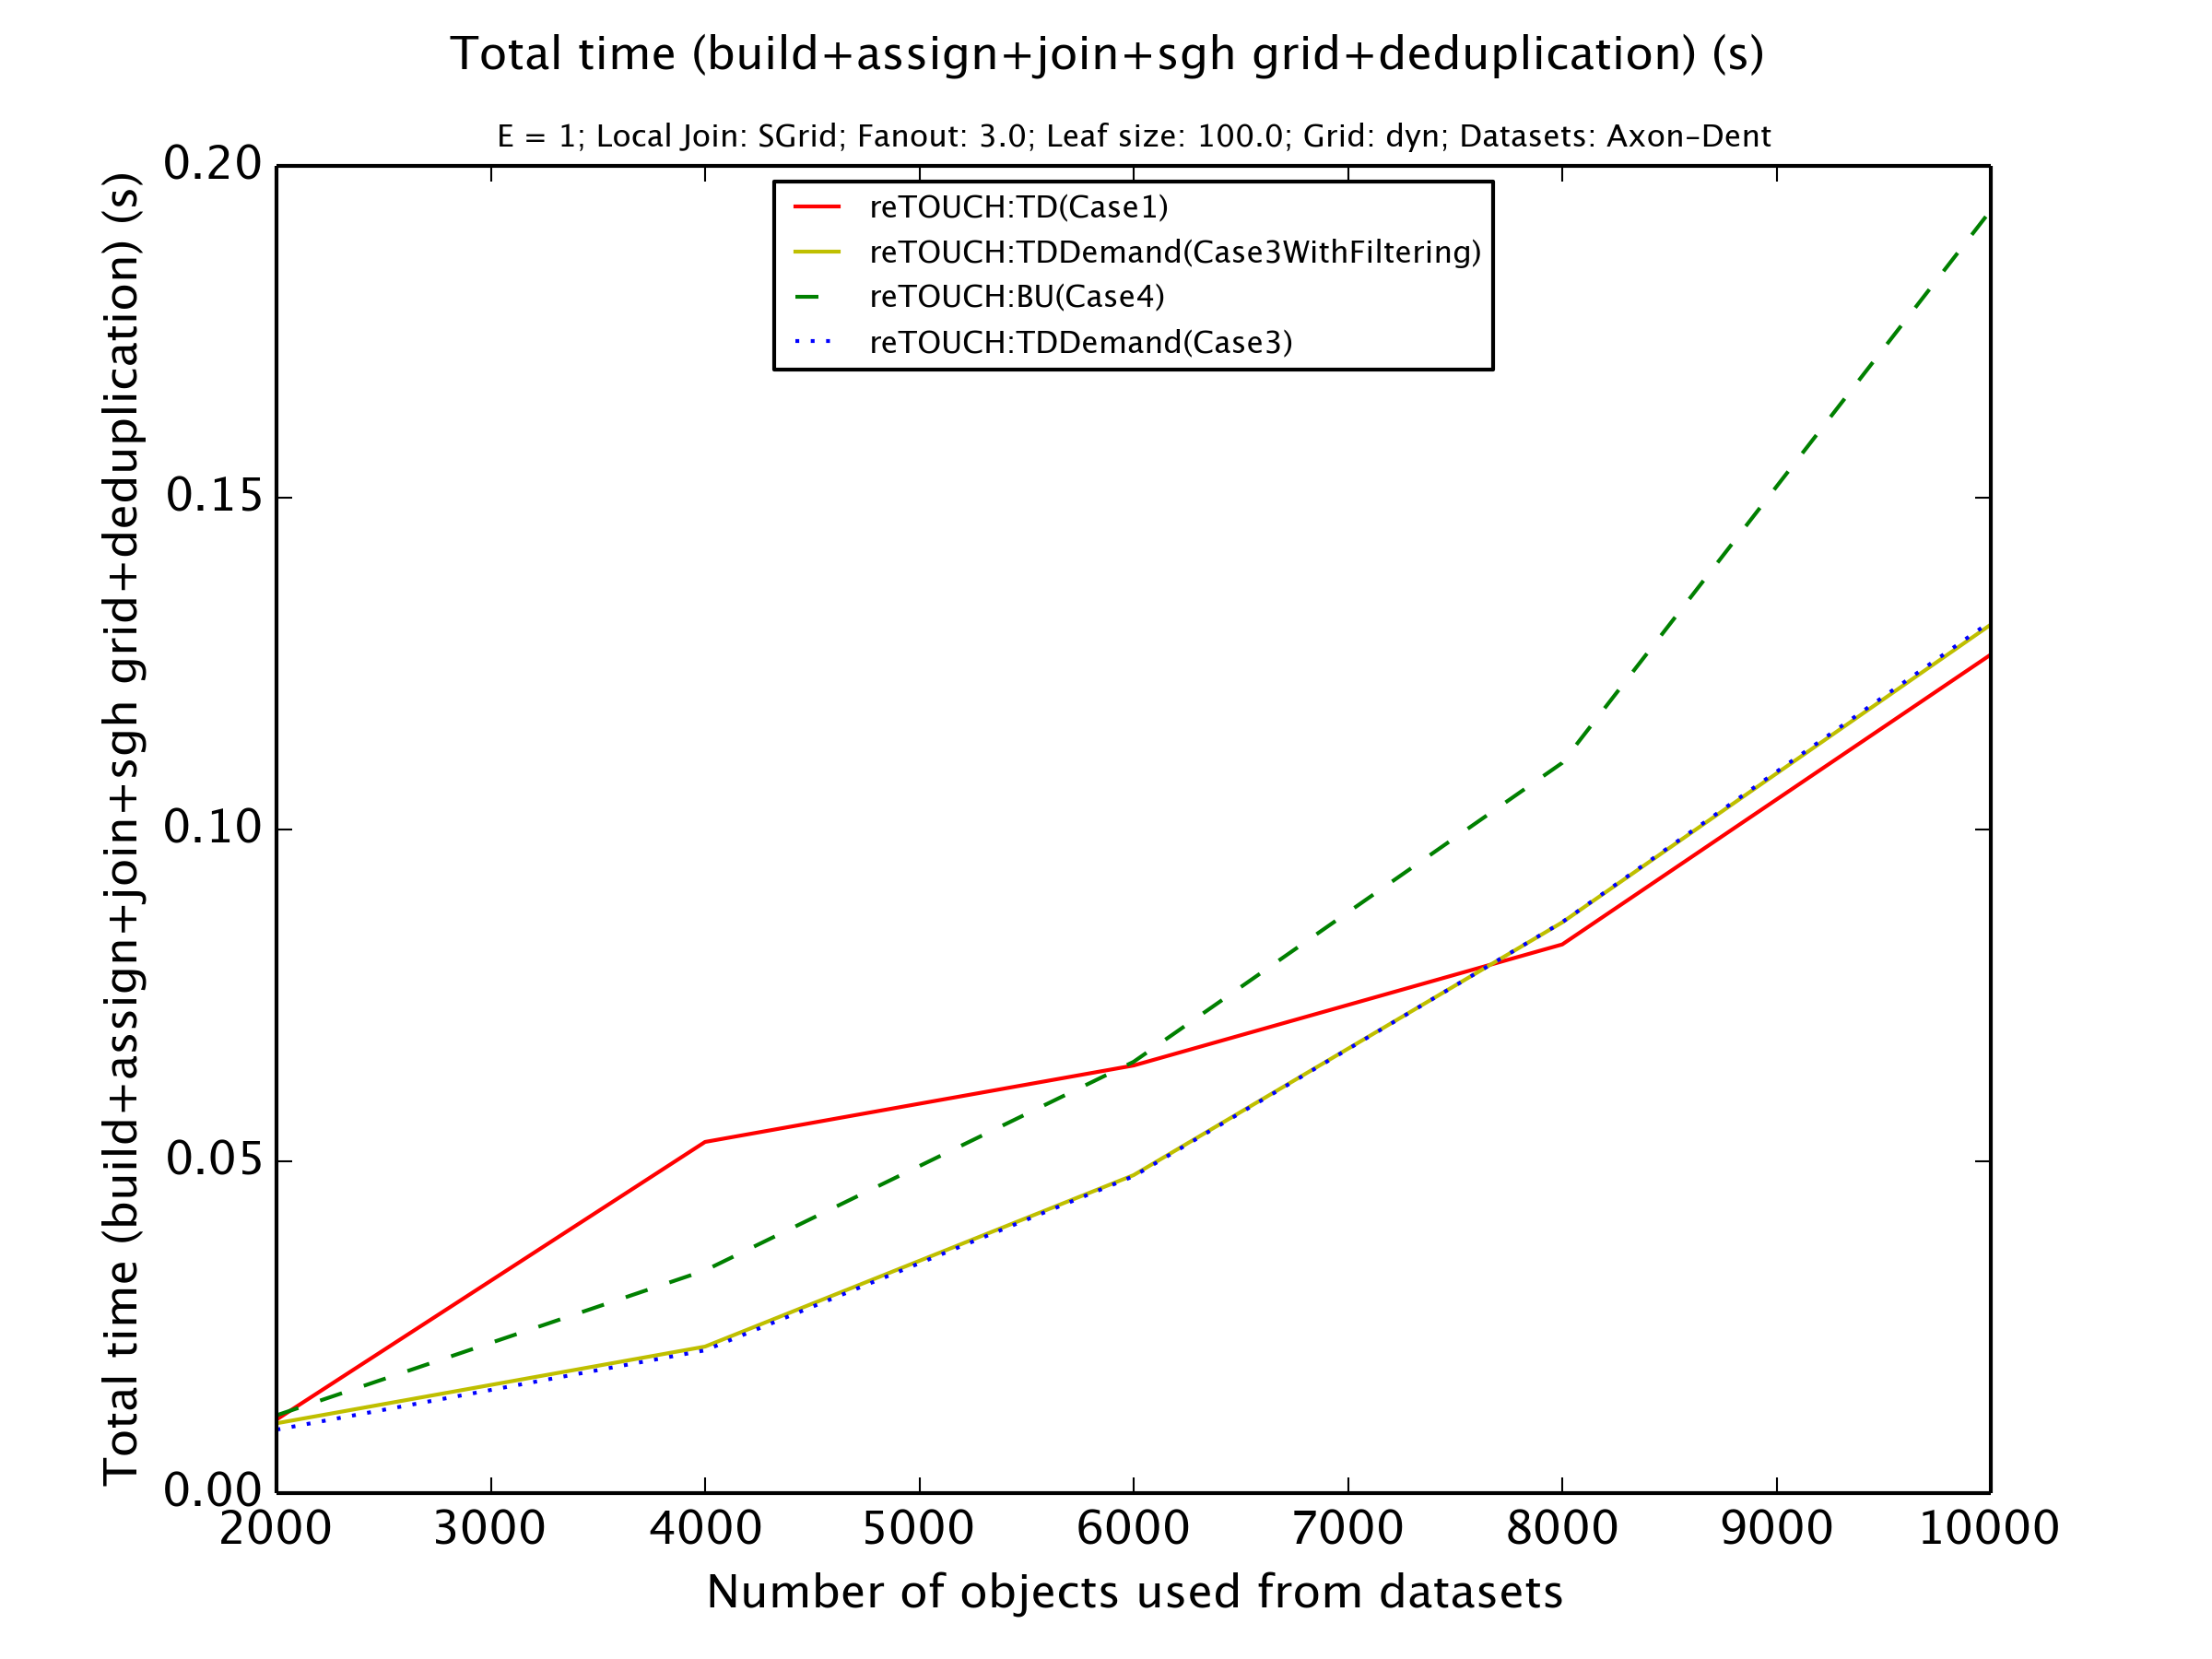
\includegraphics[width=\columnwidth]{traversalTypeFixed/total}
        \caption{Traversal type comparison: Total time}
        \label{fig:traversal:total}
      \end{center}
\end{figure}

\begin{figure}[htb]
    \begin{center}
        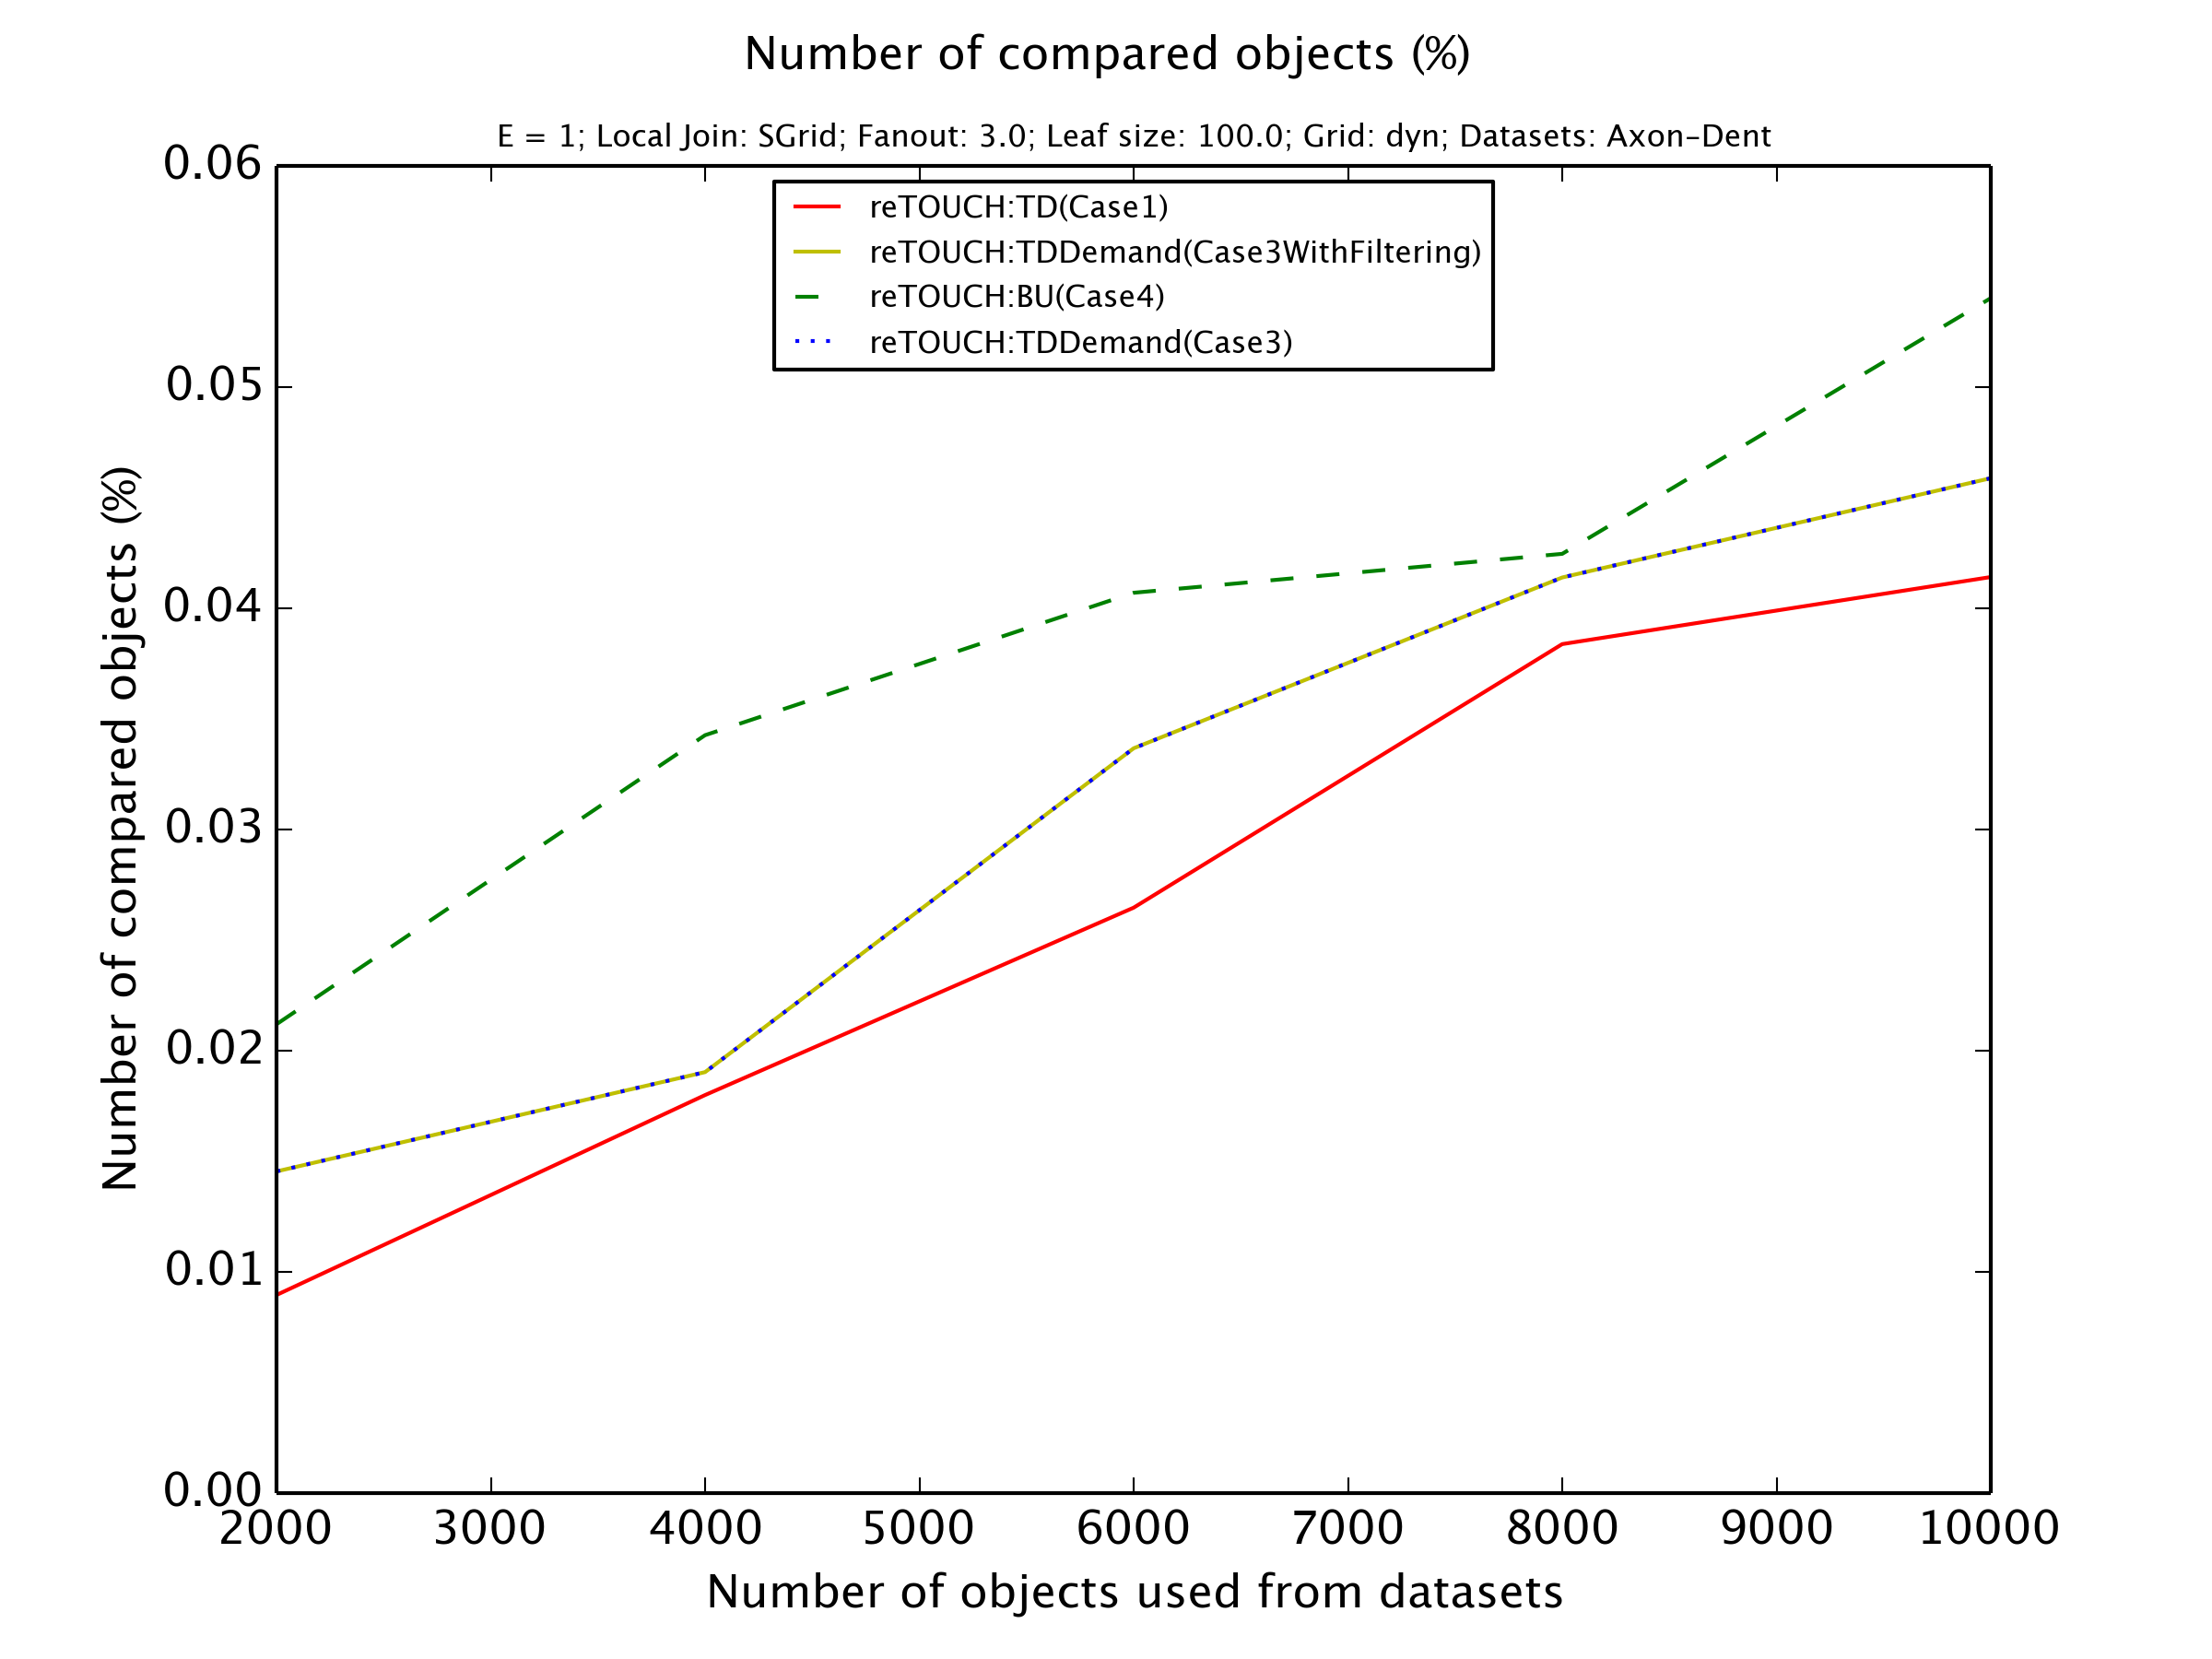
\includegraphics[width=\columnwidth]{traversalTypeFixed/objnum}
        \caption{Traversal type comparison: Number of compared objects (\%)}
        \label{fig:traversal:objnum}
      \end{center}
\end{figure}

\begin{figure}[htb]
    \begin{center}
        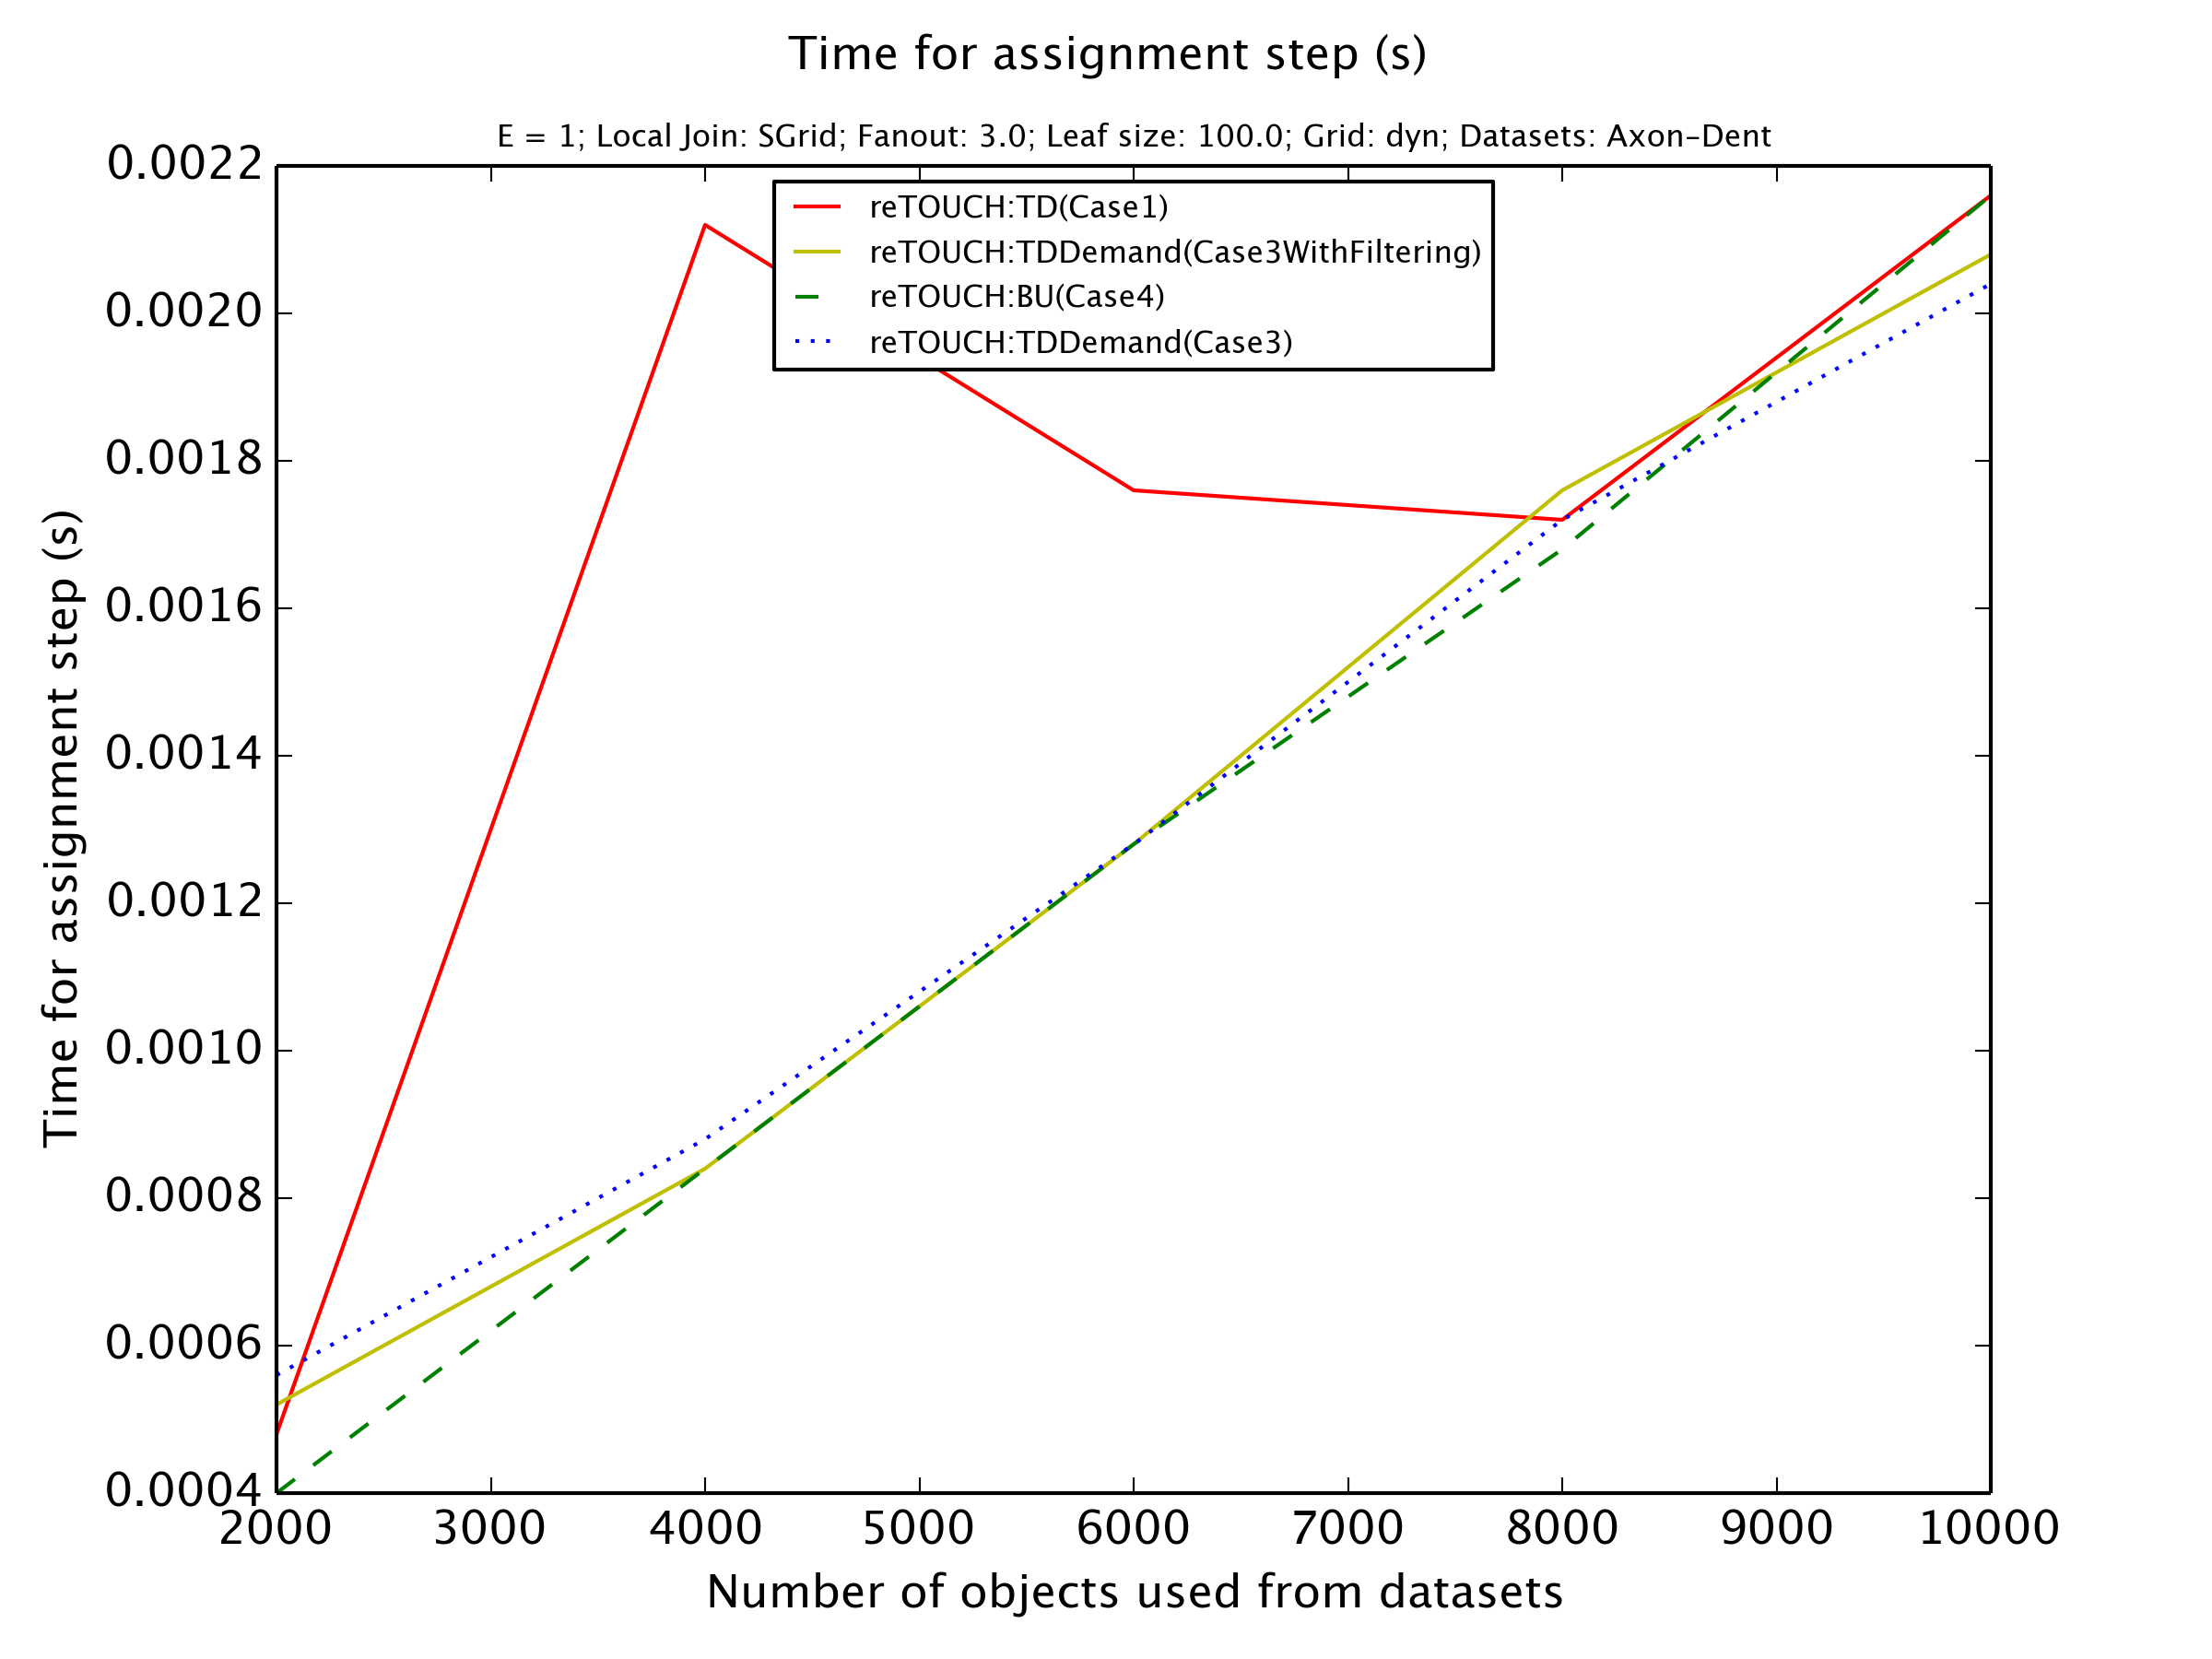
\includegraphics[width=\columnwidth]{traversalTypeFixed/assignment}
        \caption{Traversal type comparison : Assignment time}
        \label{fig:traversal:assignment}
      \end{center}
\end{figure}

\begin{figure}[htb]
    \begin{center}
        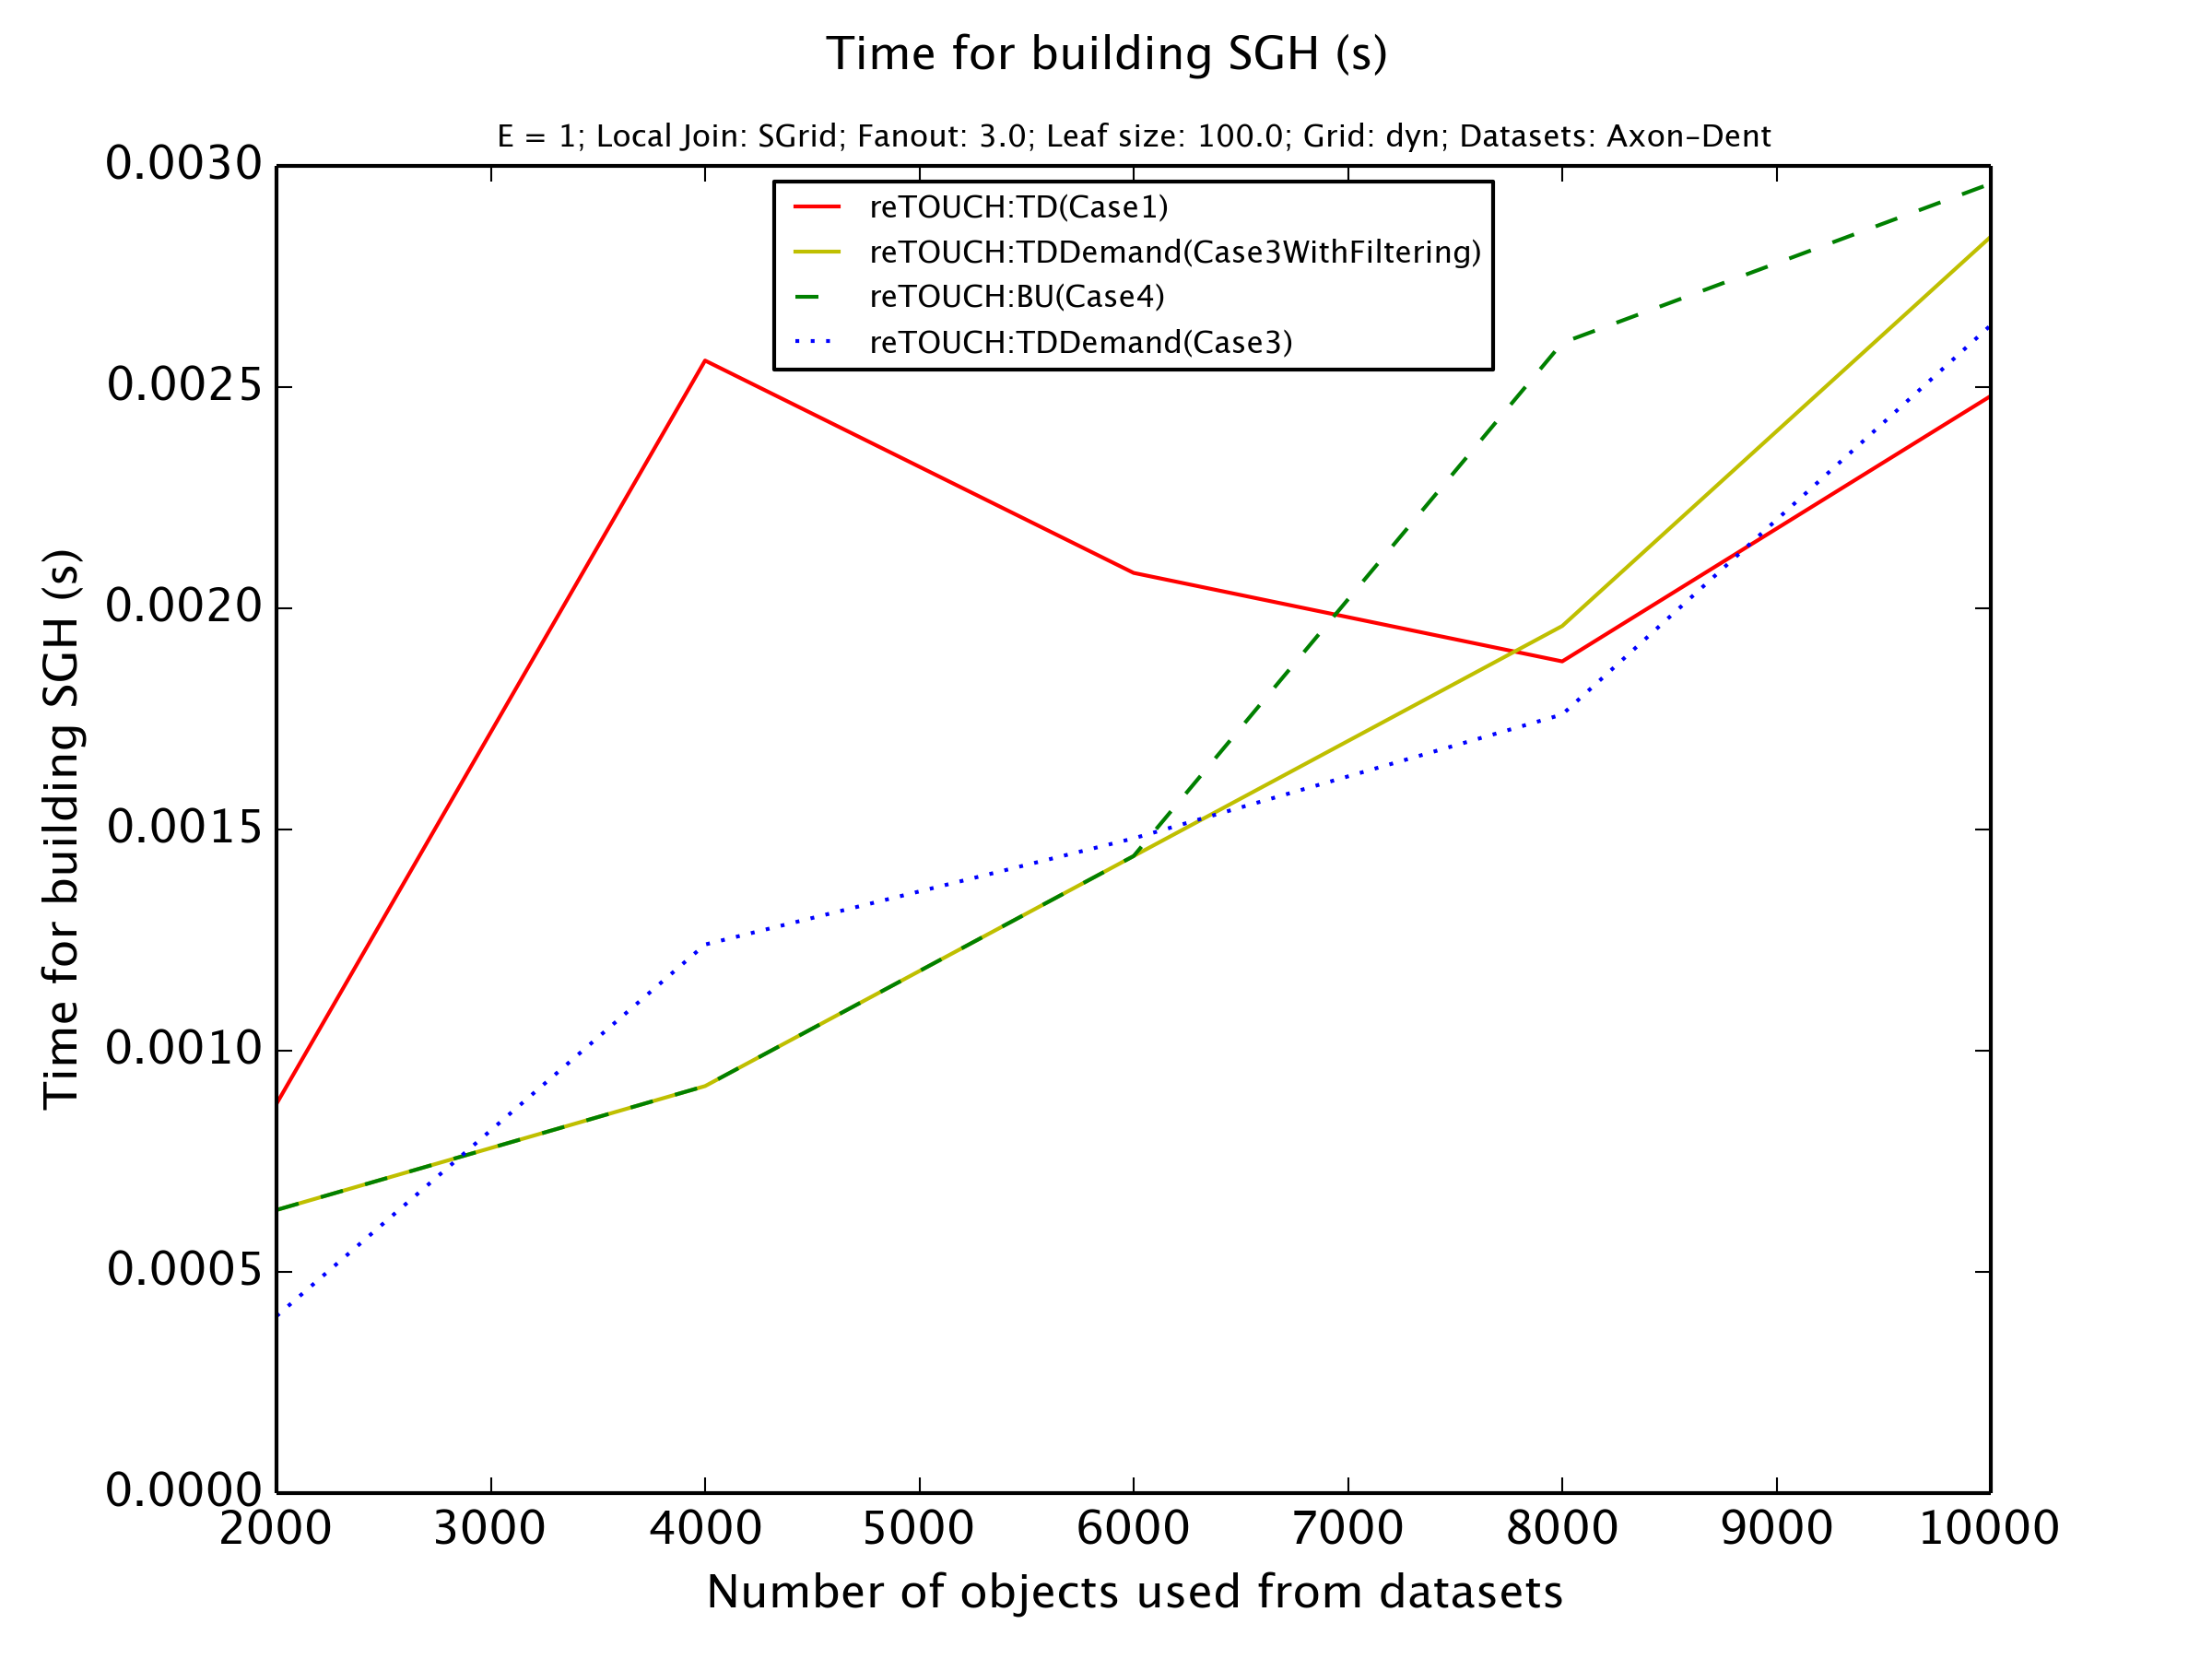
\includegraphics[width=\columnwidth]{traversalTypeFixed/building}
        \caption{Traversal type comparison : SGH builind time}
        \label{fig:traversal:sghbuild}
      \end{center}
\end{figure}

\begin{figure}[htb]
    \begin{center}
        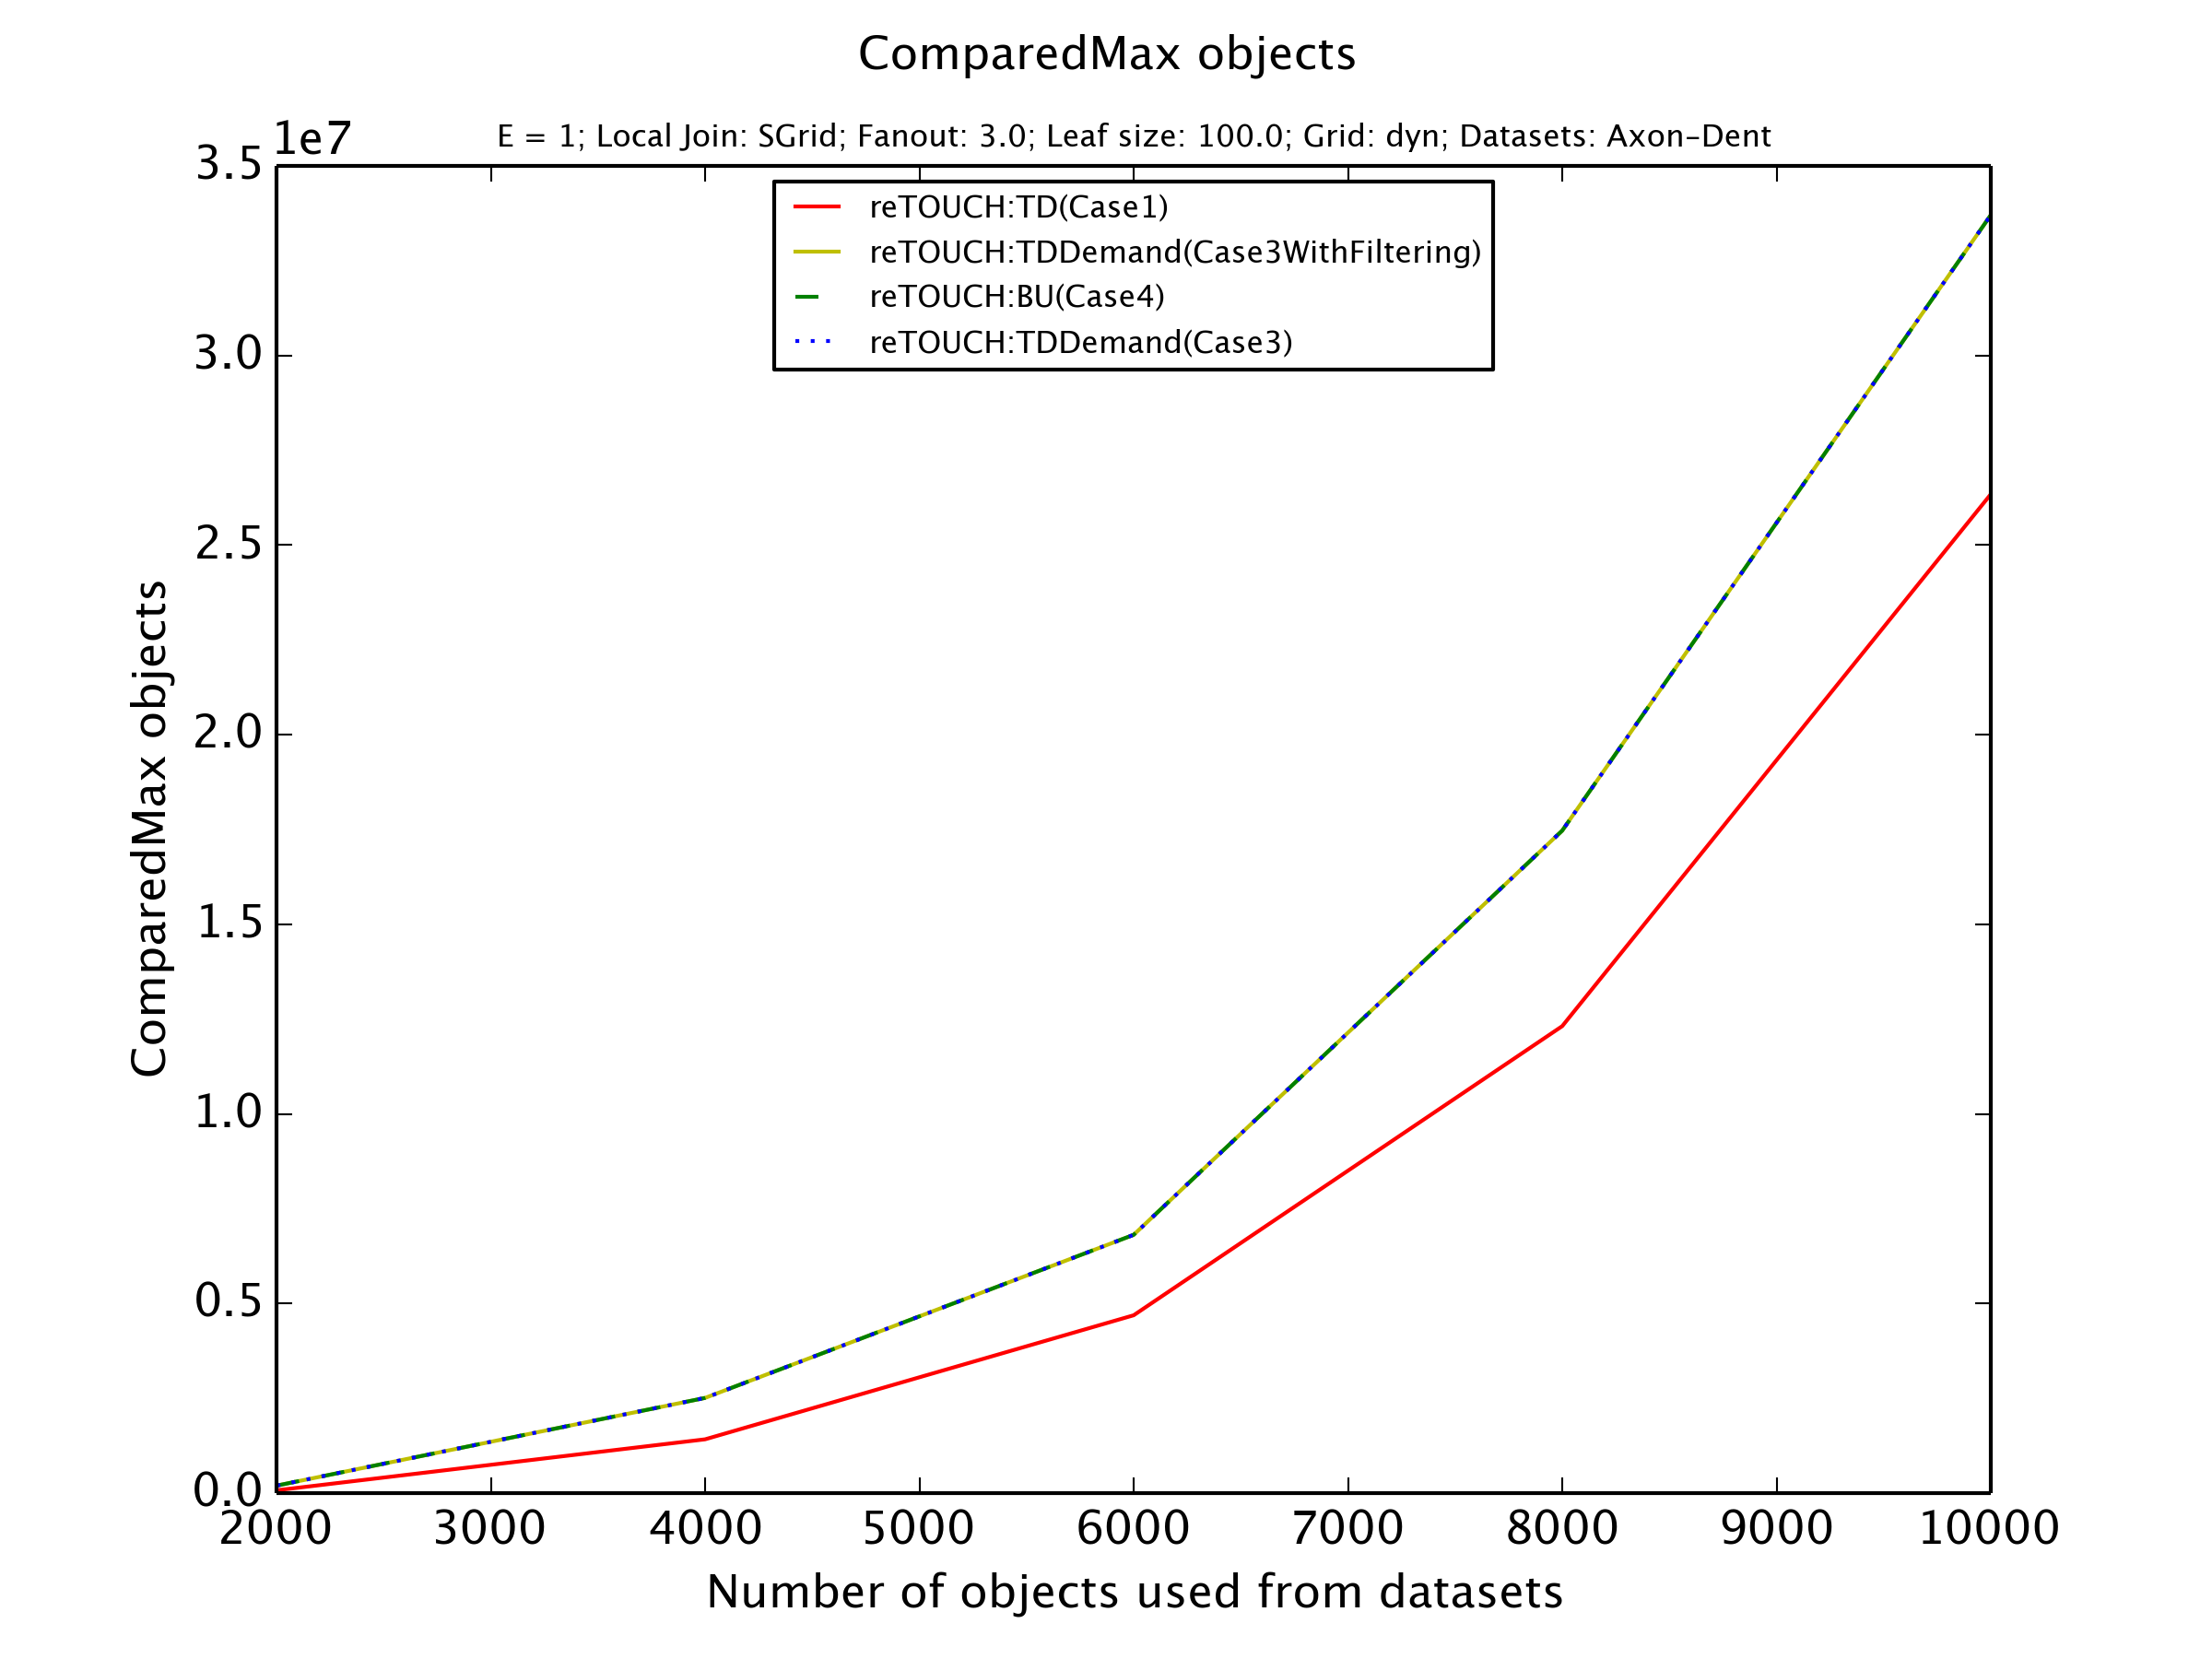
\includegraphics[width=\columnwidth]{traversalTypeFixed/NLjoin}
        \caption{Traversal type comparison : Number of compared objects if NL is used}
        \label{fig:traversal:compmax}
      \end{center}
\end{figure}

\begin{figure}[htb]
    \begin{center}
        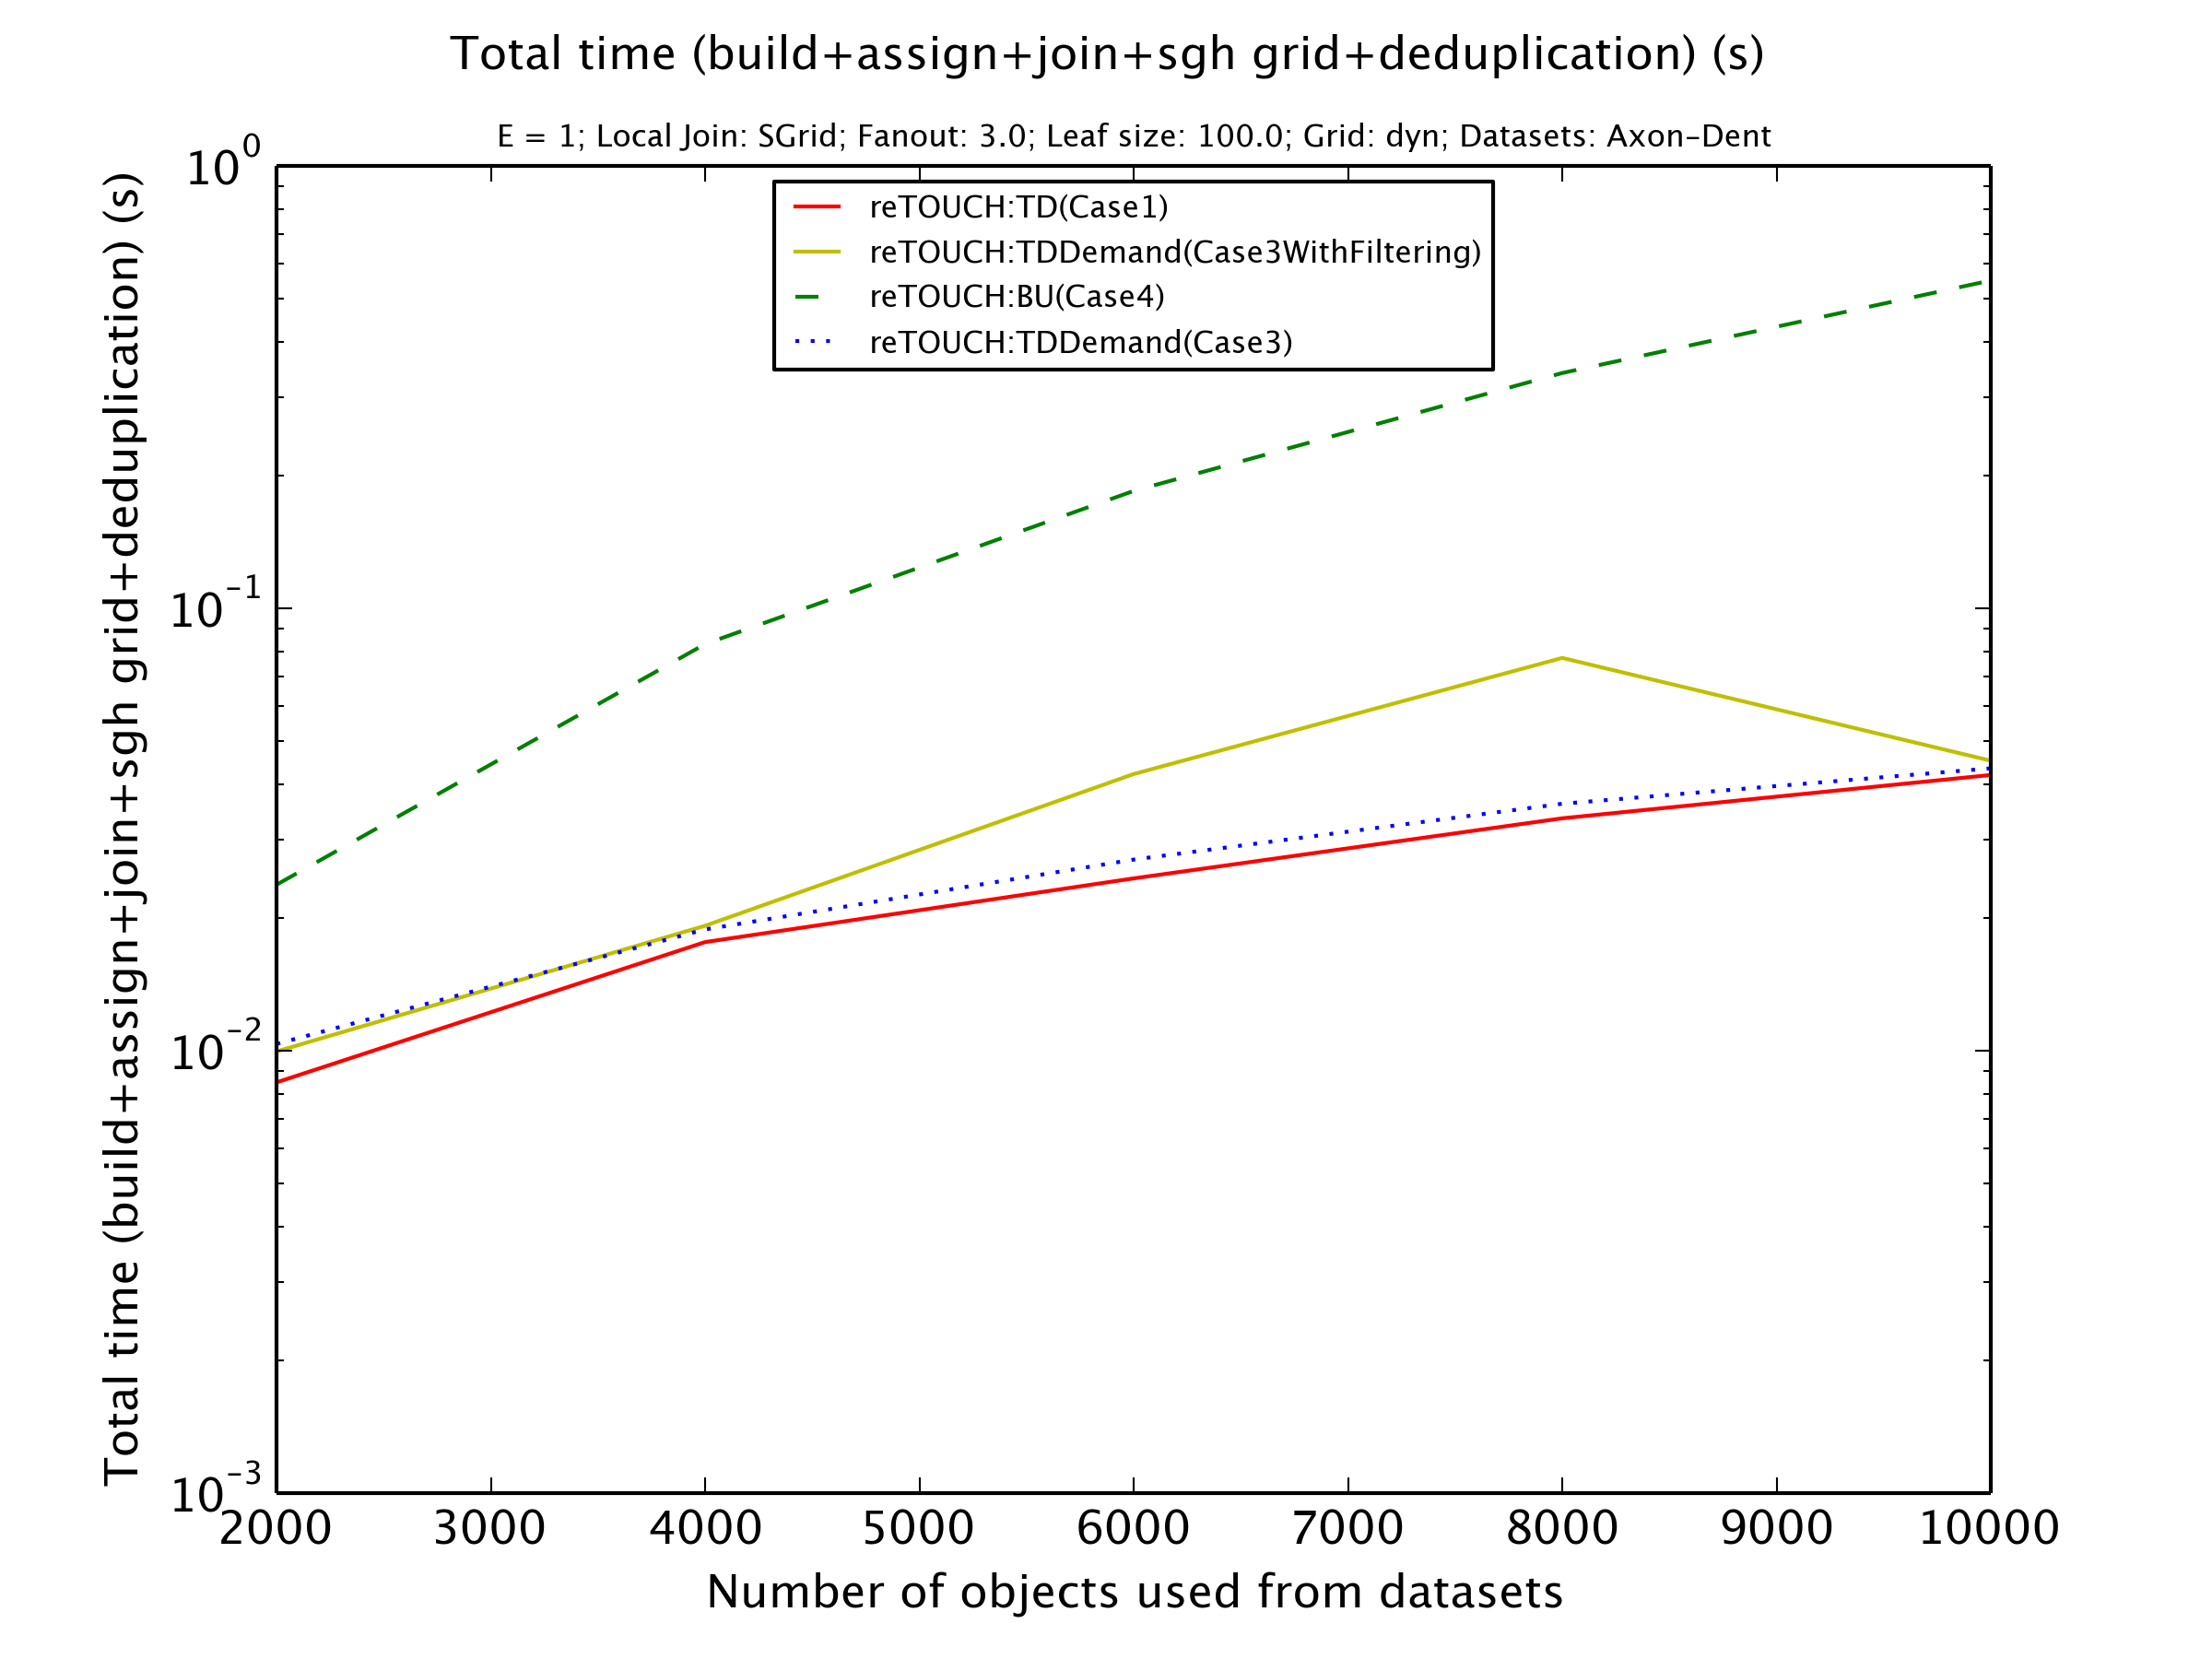
\includegraphics[width=\columnwidth]{traversalTypeWithConstantGridFixed/total}
        \caption{Traversal type comparison : Total time of joining Axon/Dendrite samples using constant SGH resolution}
        \label{fig:traversal:totalconst}
      \end{center}
\end{figure}

\begin{figure}[htb]
    \begin{center}
        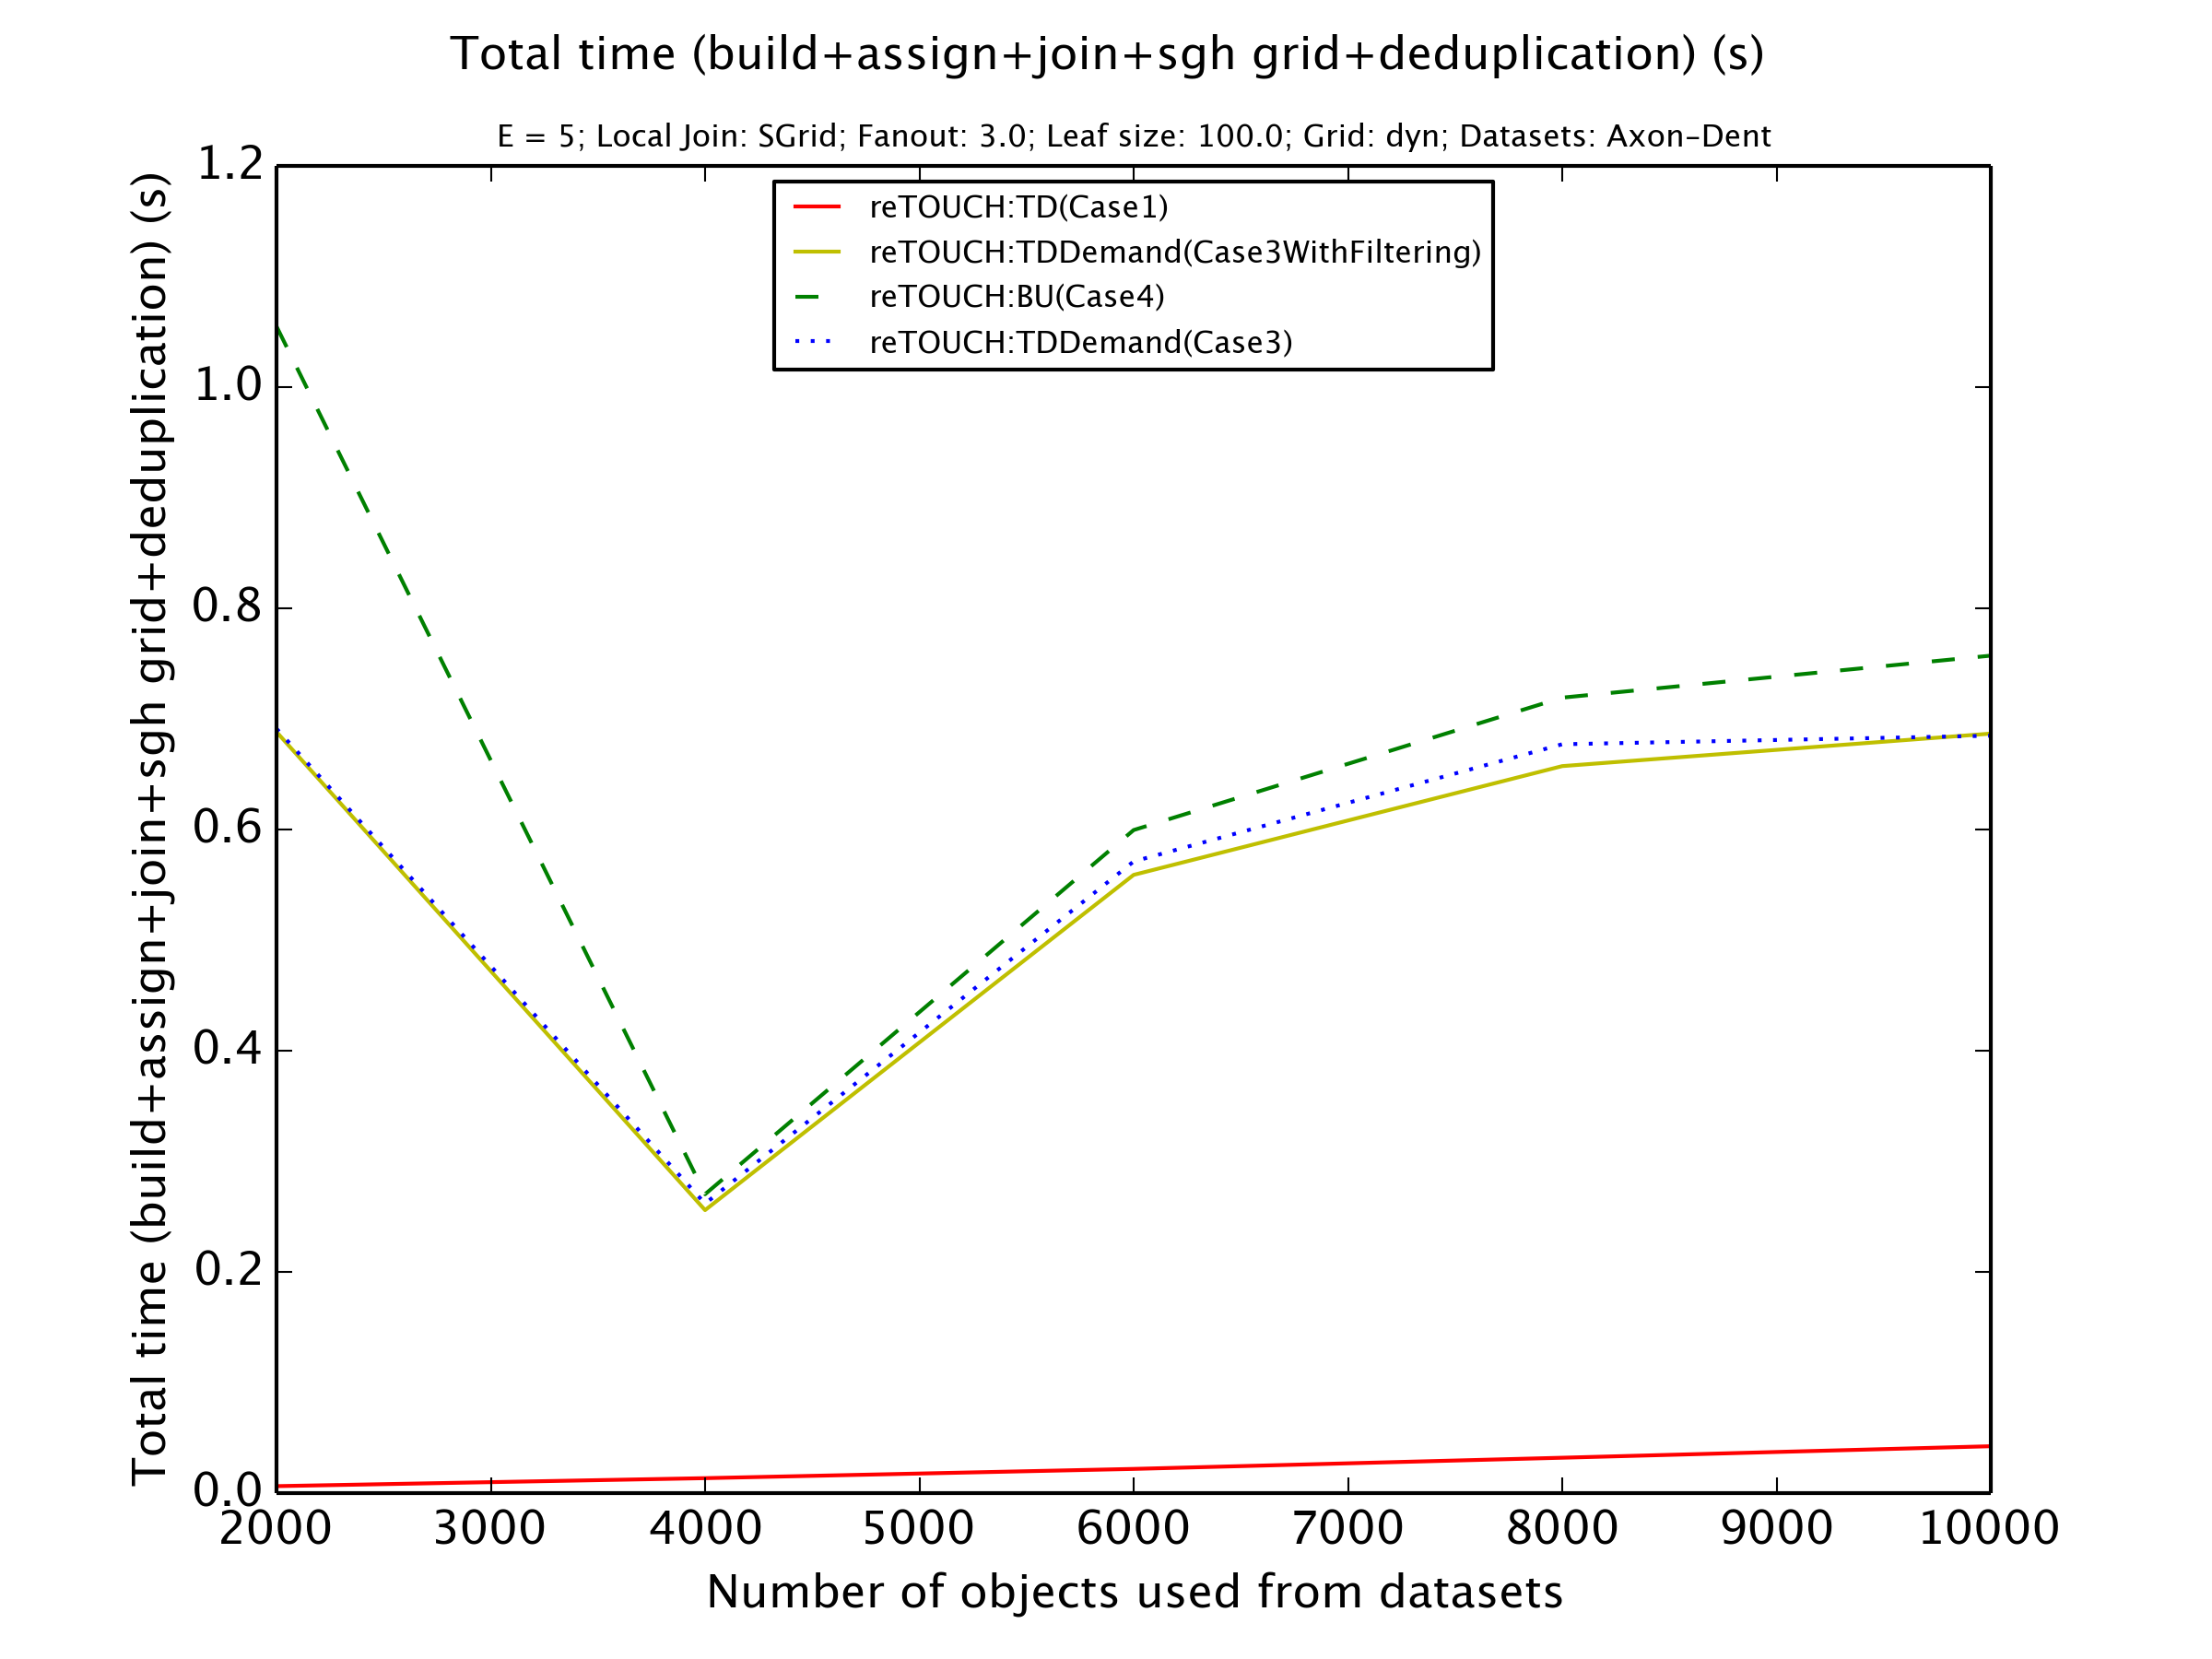
\includegraphics[width=\columnwidth]{traveralTypeRandomSizeConstantGrid/total}
        \caption{Traversal type comparison : Total time of joining UniRandomExpended samples}
        \label{fig:traversal:totalrand}
      \end{center}
\end{figure}

\subsubsection{Conclusion}
Case 1 is suggested for further experiments.

\section{Experiment terminologies}

\begin{table*}
\centering
\begin{tabular}{ |l|l| }
  \hline
  \multicolumn{2}{|c|}{Terminology table} \\
  \hline
Algorithm	& Main algorithm name\\
Epsilon		& Distance between objects such that closer objects are considered as interacting\\
\#A		& Number of objects used from first dataset\\
\#B		& Number of objects used from second dataset\\
infile A	& Path to first dataset\\
infile B	& Path to second dataset\\
LocalJoin Alg	& Algorithm used for local join (join inside nodes)\\
Fanout		& Fanout (capacity) of a node in a tree\\
Leaf size	& Size (fanout) of leaf nodes\\
gridSize	& Number of cells per dimention for Grid Hash (Local Join).\\ Resolution & $gridSize/Universe$ (all used sapce)\\
Compared \#	& Total number of comparisons (comparison function calls)\\
Compared \%	& Compared \# / (\#A*\#B) * 100\%\\
ComparedMax	& Compared \# in case of using Nested Loop as local join algorithm\\
Duplicates	& Number of duplicate result pairs in case of Grid Hash\\
Results		& Number of interacting pairs\\
Selectivity	& Results / (\#A*\#B) * 100\%\\
$F_A$	& Number of filtered objects of first dataset\\
$F_B$	& Number of filtered objects of second dataset\\
$F_total$	& $F_A + F_B$\\
t loading	& Time for loading and parsing data\\
t init		& Time for initializing Grid Hash\\
t build		& Time for assignment steps\\
t probe		& Time for probing function, total joining step\\
t comparing	& Time for Local Joins\\
t partition	& Time for creating nodes\\
t total		& Total time of Spatial Join class existance (including I/O)\\
t deDuplicating	& Time for removing duplicate objects in Grid Hash\\
t analyzing	& Time for analyzing a tree structure after assignment step\\
t sorting	& Time used for sorting objects during creation of tree structure\\
t gridCalculate	& Time for precalculating all Grid Hash for every node (cTOUCH, re*TOUCH)\\
t sizeCalculate	& Time for calculating size statistics on the nodes\\
EmptyCells(%)	& Number of nodes without objects / Total number of nodes * 100% (@todo incorrect for complex trees)\\
MaxObj		& Number of maximum assigned objects of one type to one node\\
AveObj		& Average number of objects in a node \\
StdObj		& Standart deviation of number of objects in a node \\
repA		& Number of replications of type A using Grid Hash (if one object is assigned to more than one cell of Grid Hash)\\
repB		& Number of replications of type B usign Grid Hash (if one object is assigned to more than one cell of Grid Hash)\\
max level   & Parameter that defines whether object is assigned to the first tree in dTOUCH\\
gridProbe   & (if SGH) time for calculating grid and probing together\\

  \hline
\end{tabular}
\caption{Terminologies used in the experiments.}
\label{table:terms}
\end{table*}

\end{document}
